%%%%%%%%%%%%%%%%%%%%%%%%%%%%%%%%%%%%%%%%%%%%%%%%%%%%%%%%%%%%%%%%%%%%%%%%
%                                                                      %
%     File: Thesis_Appendix_C.tex                                      %
%     Tex Master: Thesis.tex                                           %
%                                                                      %
%     Author: Andre C. Marta                                           %
%     Last modified :  2 Jul 2015                                      %
%                                                                      %
%%%%%%%%%%%%%%%%%%%%%%%%%%%%%%%%%%%%%%%%%%%%%%%%%%%%%%%%%%%%%%%%%%%%%%%%

\chapter{Miscellaneous}
\label{chapter:annexData}

\section{Traversability maps}
\label{section:traversabilityMaps}

\begin{figure}[!ht]
    \centering
	\begin{subfigmatrix}{3}
	\subfigure[Algorithm \ref{alg:slopeMinHeightMap}, where $\yaw = 0$] {
    	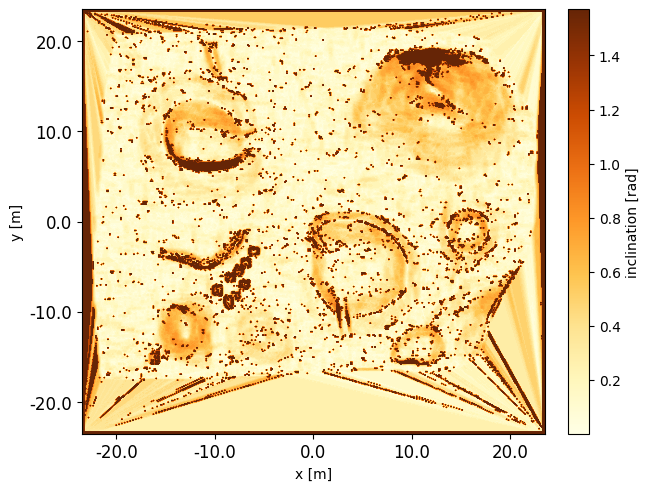
\includegraphics[width=0.31\linewidth]{Figures/HeightMin+Surface+1.png}  
	}
	\subfigure[Algorithm \ref{alg:slopeMinHeightMapVarYaw}] {
    	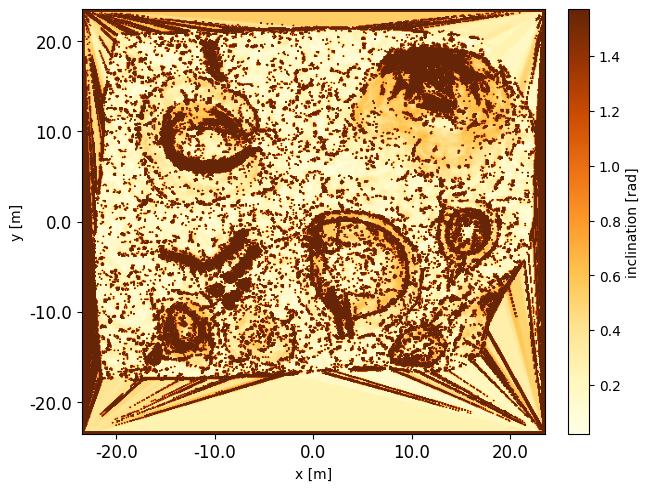
\includegraphics[width=0.31\linewidth]{Figures/HeightMin_maxInclination+Surface+1.png}  
	}
	\subfigure[Algorithm \ref{alg:maxRoughnessMap}] {
    	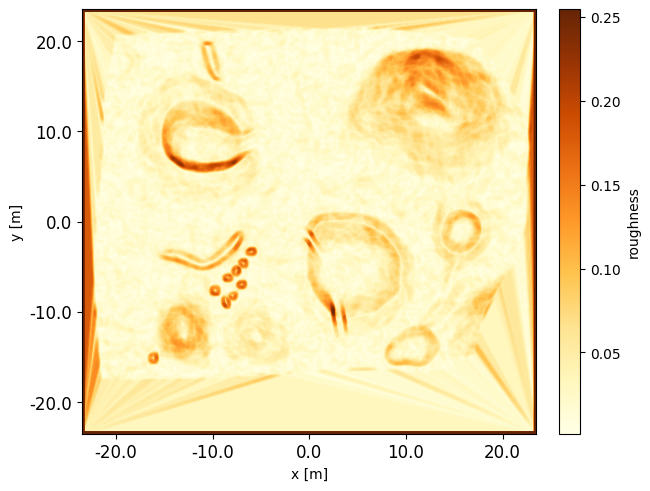
\includegraphics[width=0.31\linewidth]{Figures/maxTerrainRoughness+1.png}  
	}
	\end{subfigmatrix}
    \caption{Traversability maps (case 2; map 1)}
    \label{fig:costMapsCase2Alg2_4}
\end{figure}

\begin{figure}[!ht]
    \centering
	\begin{subfigmatrix}{2}
	\subfigure[Worst-case map] {
    	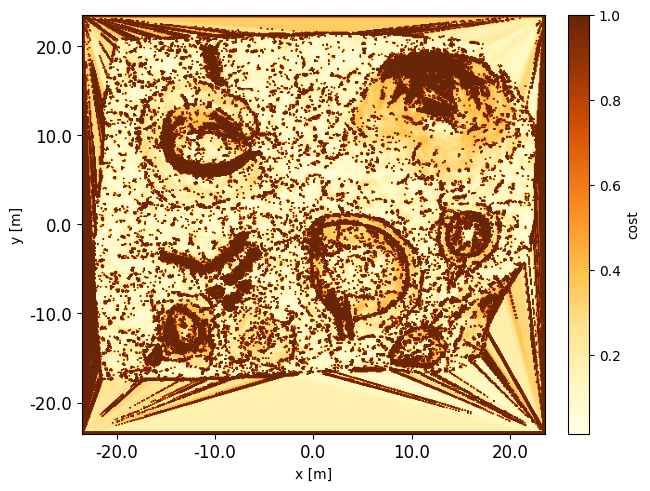
\includegraphics[width=0.48\linewidth]{Figures/worstCase+Surface+1.png}  
	}
	\subfigure[Algorithm \ref{alg:refinedMap}, where $r_s$ = 0.2 m and $C$ = 0.9] {
    	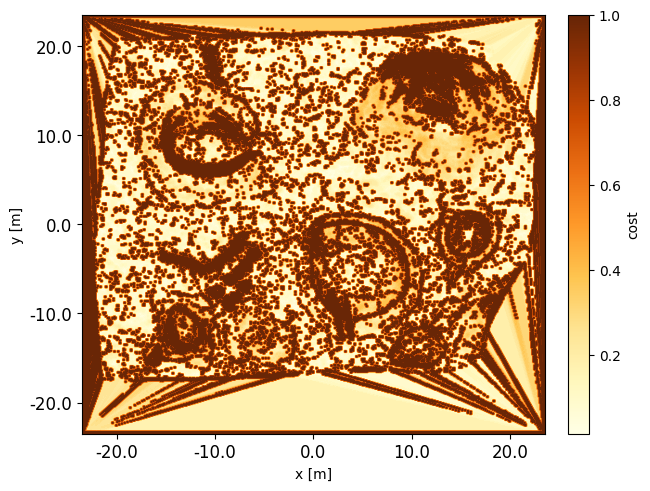
\includegraphics[width=0.48\linewidth]{Figures/mapRefinement+Surface+0.9+0.2+1.png}  
	}
	\end{subfigmatrix}
    \caption{Traversability maps (case 2; map 1)}
    \label{fig:costMapsCase2Alg5}
\end{figure}

\section{Performance metrics of controllers}
\label{section:performanceMetrics}

For the sake of brevity and space saving in this document, the performance metrics of controllers are presented below.

\subsection{One-stage planar \acrshort{ocp}}
\label{subsection:onestageplanarocp}

The performance metrics presented in this subsection concern the results discussed in subsection \ref{subsection:solverspecssurvey}.

\subsubsection*{Control horizon}

\begin{table}[!htb]
  \caption[Cumulative control effort of controllers when control horizon changes.]{Cumulative control effort $[N \cdot s]$.}
  \label{tab:cumulativeControlEffortControlHorizon}
  \renewcommand{\arraystretch}{1.2} % more space between rows
  \centering
  \begin{tabular}{lccccc}
    \toprule
     & $N = 10$ & $N = 20$ & $N = 30$ & $N = 50$ & $N = 100$ \\
    \midrule
    $\left(a\right)$ & $44.11$ & $46.14$ & $47.32$ & $44.82$ & $45.50$ \\
    $\left(b\right)$ & $50.64$ & $51.03$ & $52.09$ & $55.88$ & $55.00$ \\
    \bottomrule
  \end{tabular}
\end{table}

\begin{table}[!htb]
  \caption[Cumulative positional error of controllers when control horizon changes.]{Cumulative positional error $[m]$.}
  \label{tab:cumulativePositionalErrorControlHorizon}
  \renewcommand{\arraystretch}{1.2}
  \centering
  \begin{tabular}{lccccc}
    \toprule
     & $N = 10$ & $N = 20$ & $N = 30$ & $N = 50$ & $N = 100$ \\
    \midrule
    $\left(a\right)$ & $366.14$ & $306.58$ & $279.74$ & $255.94$ & $246.12$ \\
    $\left(b\right)$ & $410.20$ & $369.43$ & $353.80$ & $384.91$ & $380.31$ \\
    \bottomrule
  \end{tabular}
\end{table}

\begin{table}[!htb]
  \caption[Cumulative heading error of controllers when control horizon changes.]{Cumulative heading error.}
  \label{tab:cumulativeHeadingErrorControlHorizon}
  \renewcommand{\arraystretch}{1.2}
  \centering
  \begin{tabular}{lccccc}
    \toprule
     & $N = 10$ & $N = 20$ & $N = 30$ & $N = 50$ & $N = 100$ \\
    \midrule
    $\left(a\right)$ & $64.91$ & $77.72$ & $84.80$ & $92.25$ & $193.79$ \\
    $\left(b\right)$ & $60.11$ & $70.18$ & $76.27$ & $174.84$ & $177.28$ \\
    \bottomrule
  \end{tabular}
\end{table}

\subsubsection*{Sampling time}

\begin{table}[!htb]
  \caption[Cumulative control effort of controllers when sampling time changes.]{Cumulative control effort $[N]$.}
  \label{tab:cumulativeControlEffortSamplingTime}
  \renewcommand{\arraystretch}{1.2} % more space between rows
  \centering
  \begin{tabular}{lccccc}
    \toprule
     & $T_s = 1\,ms$ & $T_s = 5\,ms$ & $T_s = 10\,ms$ & $T_s = 20\,ms$ & $T_s = 100\,ms$ \\
    \midrule
    $\left(a\right)$ & $36850.52$ & $5843.68$ & $4732.39$ & $3838.71$ & $3549.30$ \\
    $\left(b\right)$ & $29865.59$ & $6865.72$ & $5209.71$ & $4655.98$ & $3887.58$ \\
    \bottomrule
  \end{tabular}
\end{table}

\begin{table}[!htb]
  \caption[Cumulative positional error of controllers when sampling time changes.]{Cumulative positional error $[m]$.}
  \label{tab:cumulativePositionalErrorSamplingTime}
  \renewcommand{\arraystretch}{1.2}
  \centering
  \begin{tabular}{lccccc}
    \toprule
     & $T_s = 1\,ms$ & $T_s = 5\,ms$ & $T_s = 10\,ms$ & $T_s = 20\,ms$ & $T_s = 100\,ms$ \\
    \midrule
    $\left(a\right)$ & $3249.56$ & $651.12$ & $279.74$ & $126.99$ & $25.76$ \\
    $\left(b\right)$ & $3209.73$ & $707.17$ & $353.79$ & $233.30$ & $253.01$ \\
    \bottomrule
  \end{tabular}
\end{table}

\begin{table}[!htb]
  \caption[Cumulative heading error of controllers when sampling time changes.]{Cumulative heading error.}
  \label{tab:cumulativeHeadingErrorSamplingTime}
  \renewcommand{\arraystretch}{1.2}
  \centering
  \begin{tabular}{lccccc}
    \toprule
     & $T_s = 1\,ms$ & $T_s = 5\,ms$ & $T_s = 10\,ms$ & $T_s = 20\,ms$ & $T_s = 100\,ms$ \\
    \midrule
    $\left(a\right)$ & $416.87$ & $144.87$ & $84.80$ & $47.46$ & $20.41$ \\
    $\left(b\right)$ & $407.51$ & $131.96$ & $76.27$ & $89.37$ & $38.27$ \\
    \bottomrule
  \end{tabular}
\end{table}

\subsubsection*{Cost function weights}

\begin{table}[!htb]
  \caption[Cumulative control effort of controllers when cost function weights changes.]{Cumulative control effort $[N \cdot s]$.}
  \label{tab:cumulativeControlEffortWeights}
  \renewcommand{\arraystretch}{1.2} % more space between rows
  \centering
  \begin{tabular}{lccccc}
    \toprule
     & (1) & (2) & (3) & (4) & (5) \\
    \midrule
    $\left(a\right)$ & $44.82$ & $42.10$ & $45.35$ & $23.75$ & $41.48$ \\
    $\left(b\right)$ & $55.88$ & $55.55$ & $55.49$ & $45.67$ & $51.80$ \\
    \bottomrule
  \end{tabular}
\end{table}

\begin{table}[!htb]
  \caption[Cumulative positional error of controllers when cost function weights changes.]{Cumulative positional error $[m]$.}
  \label{tab:cumulativePositionalErrorWeights}
  \renewcommand{\arraystretch}{1.2}
  \centering
  \begin{tabular}{lccccc}
    \toprule
     & (1) & (2) & (3) & (4) & (5) \\
    \midrule
    $\left(a\right)$ & $255.94$ & $224.08$ & $309.85$ & $304.24$ & $261.74$ \\
    $\left(b\right)$ & $384.91$ & $387.25$ & $390.92$ & $510.10$ & $391.27$ \\
    \bottomrule
  \end{tabular}
\end{table}

\begin{table}[!htb]
  \caption[Cumulative heading error of controllers when cost function weights changes.]{Cumulative heading error.}
  \label{tab:cumulativeHeadingErrorWeights}
  \renewcommand{\arraystretch}{1.2}
  \centering
  \begin{tabular}{lccccc}
    \toprule
     & (1) & (2) & (3) & (4) & (5) \\
    \midrule
    $\left(a\right)$ & $92.25$ & $117.63$ & $70.44$ & $108.00$ & $90.72$ \\
    $\left(b\right)$ & $174.84$ & $186.69$ & $162.88$ & $192.66$ & $174.55$ \\
    \bottomrule
  \end{tabular}
\end{table}

\begin{figure}[!htb]
	\centering
	\subfigure[Controlled virtual speed inside \acrshort{ocp}]{
        \centering
        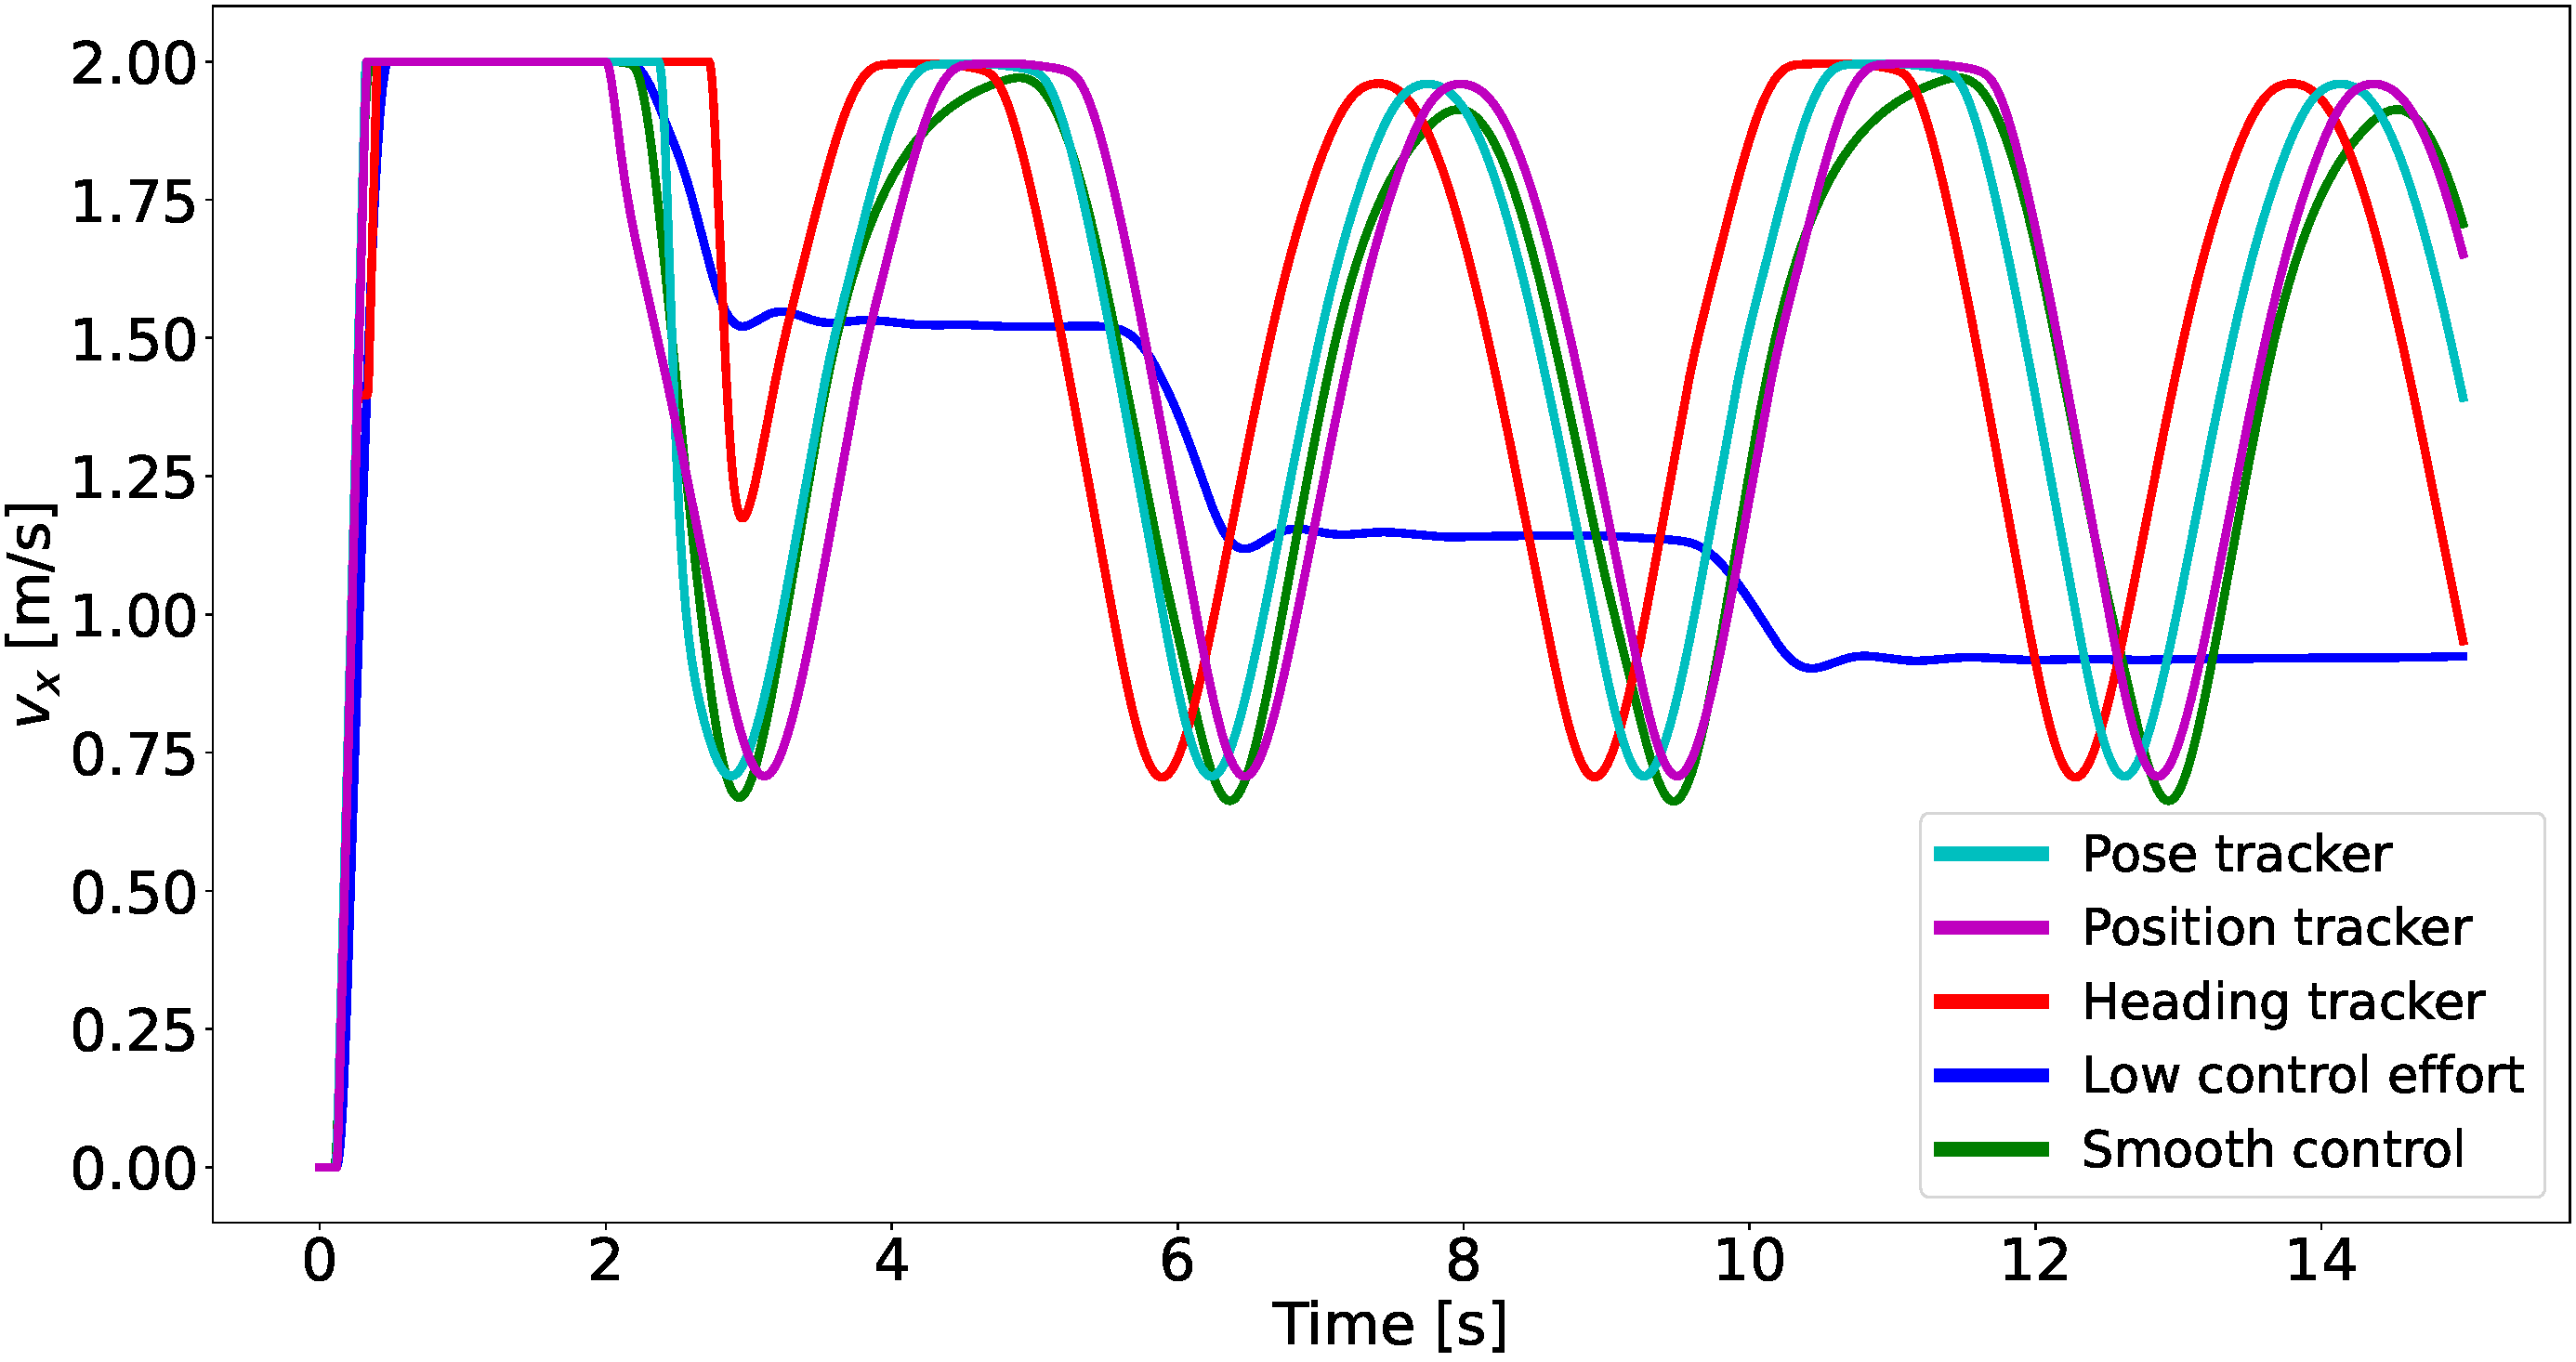
\includegraphics[width=0.48\textwidth]{Figures/One stage OCP/Solver specs comparison/Weights/Virtual speed controlled inside OCP/Planar_onestage_ocp_control_vspeed_comp_vx_weights.pdf}
        \label{subfig:PathTrackCompWeightsVarInsideVspeed_tl}
	}
	\hspace{-1.0em}
    \subfigure[Controlled virtual speed outside \acrshort{ocp}]{
        \centering
        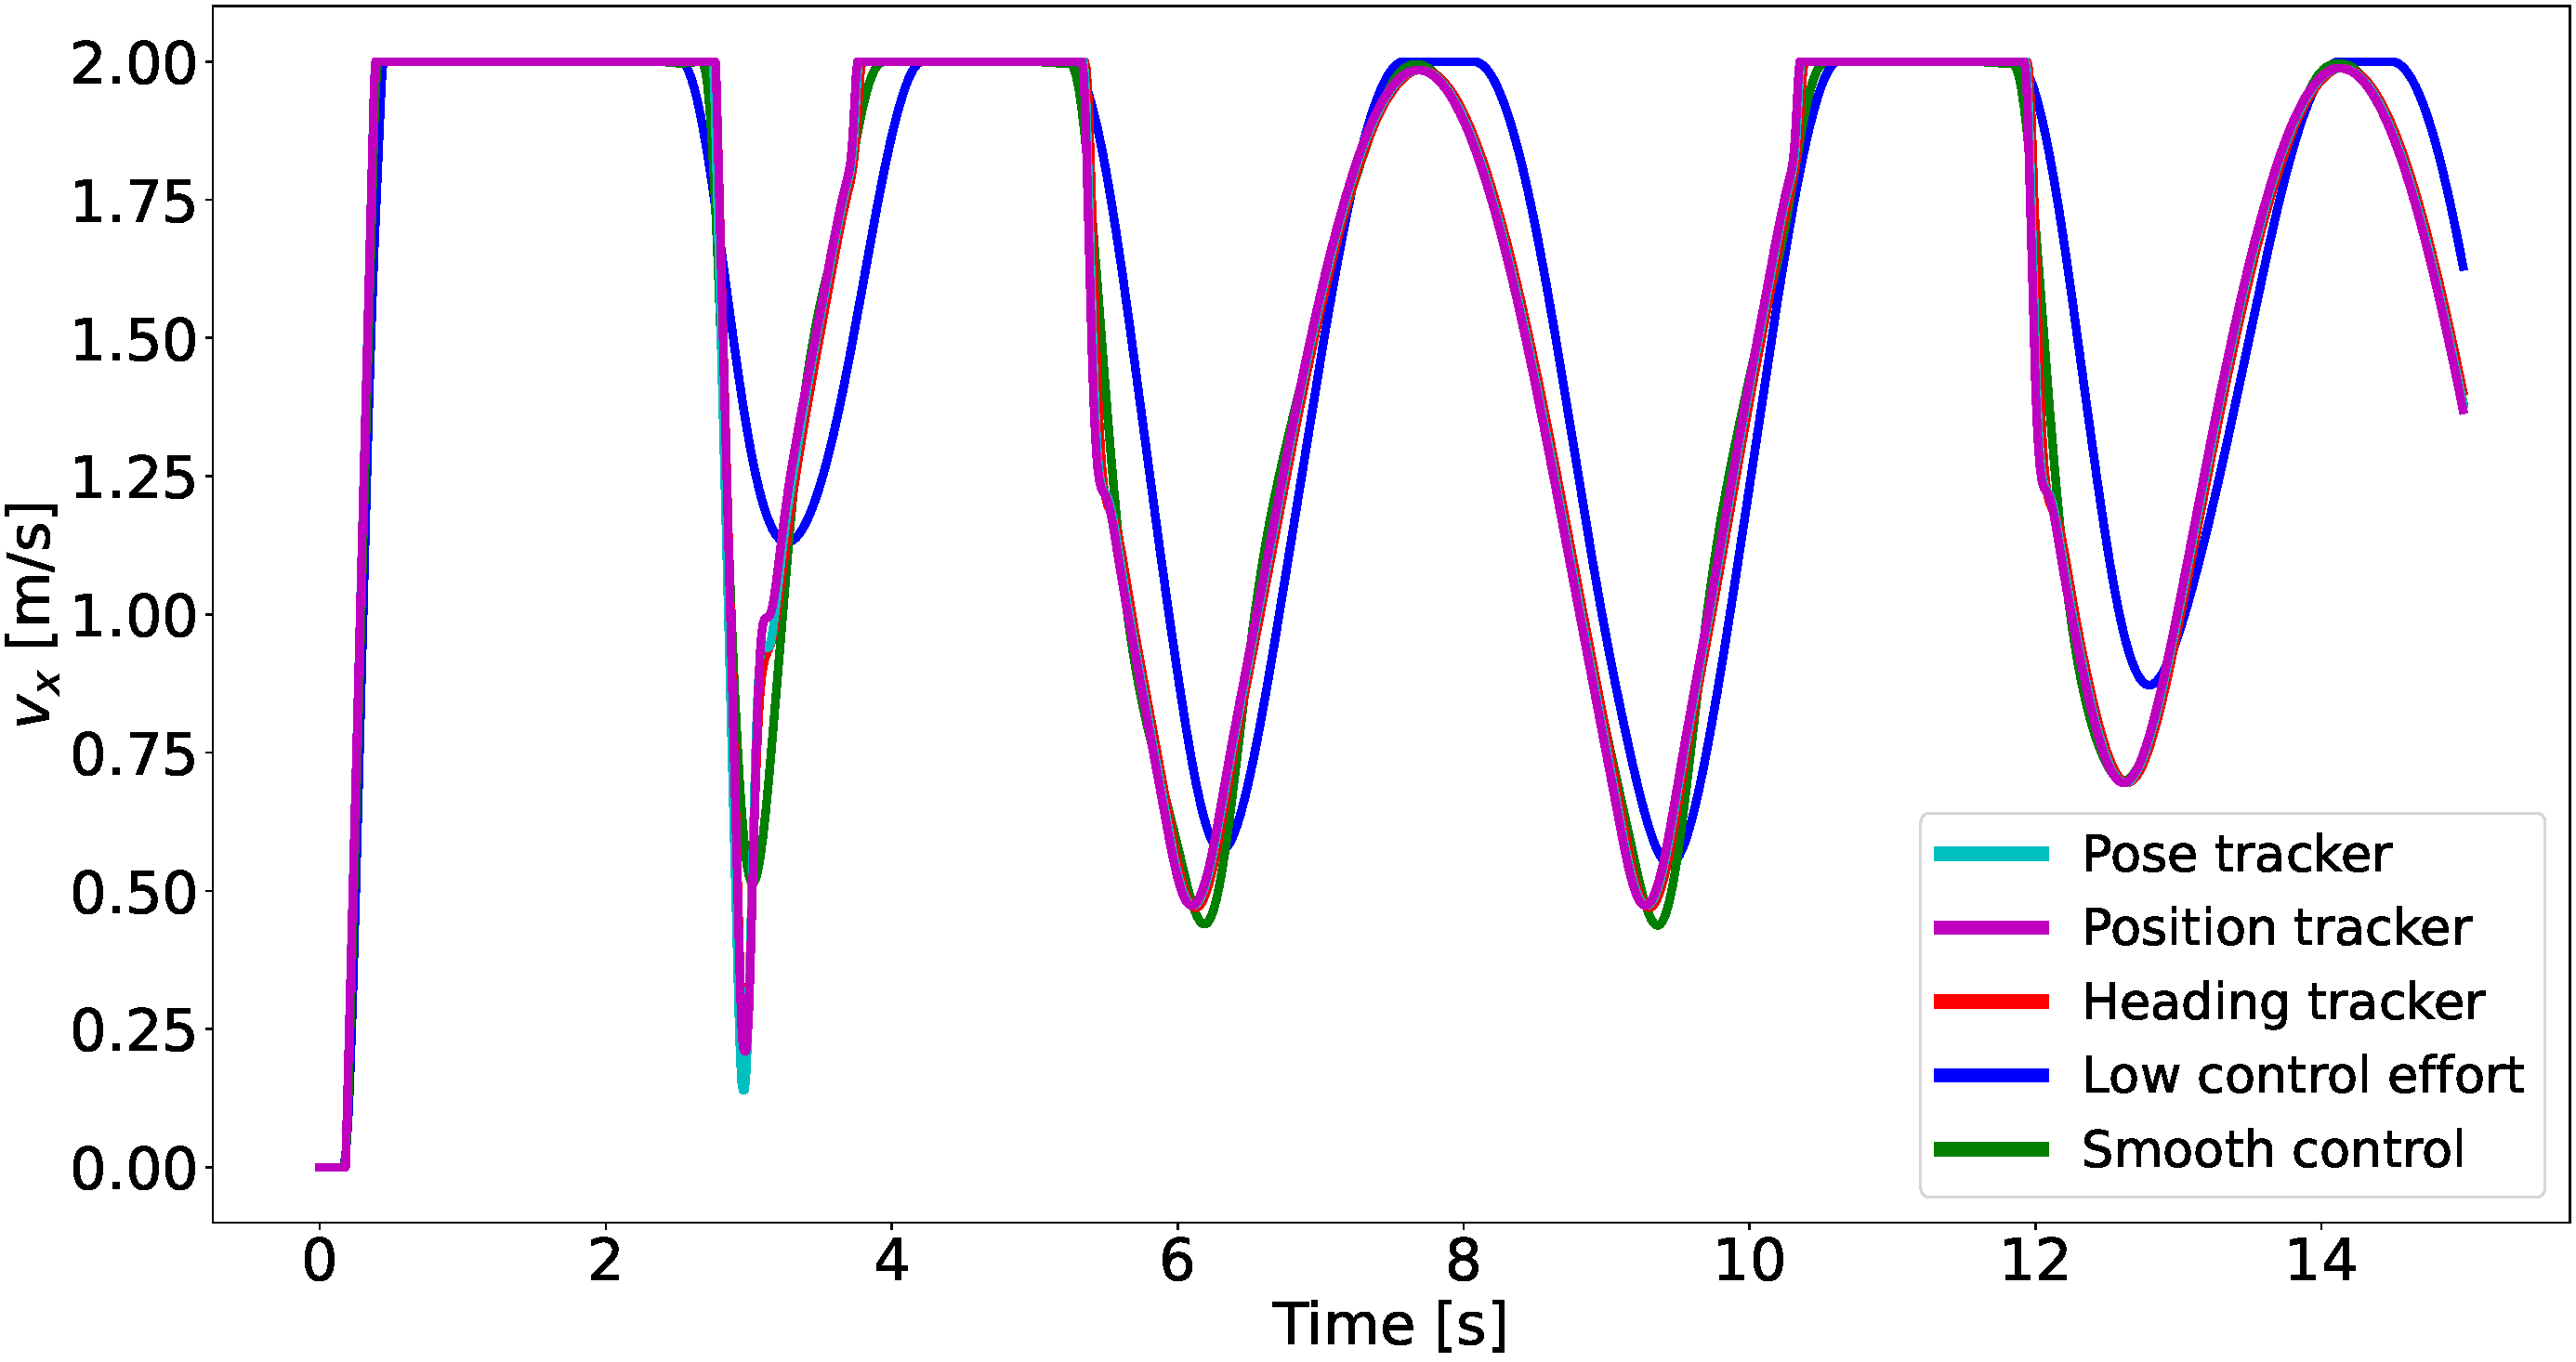
\includegraphics[width=0.48\textwidth]{Figures/One stage OCP/Solver specs comparison/Weights/Virtual speed controlled outside OCP/Planar_onestage_ocp_control_outside_vspeed_comp_vx_weights.pdf}
        \label{subfig:PathTrackCompWeightsVarOutsideVspeed_tl}
	}
	\caption{$v_x$ curve comparison among controllers.}
	\label{fig:PathTrackCompWeightsVar_vx}
\end{figure}

\begin{figure}[!htb]
	\centering
	\subfigure[Controlled virtual speed inside \acrshort{ocp}]{
        \centering
        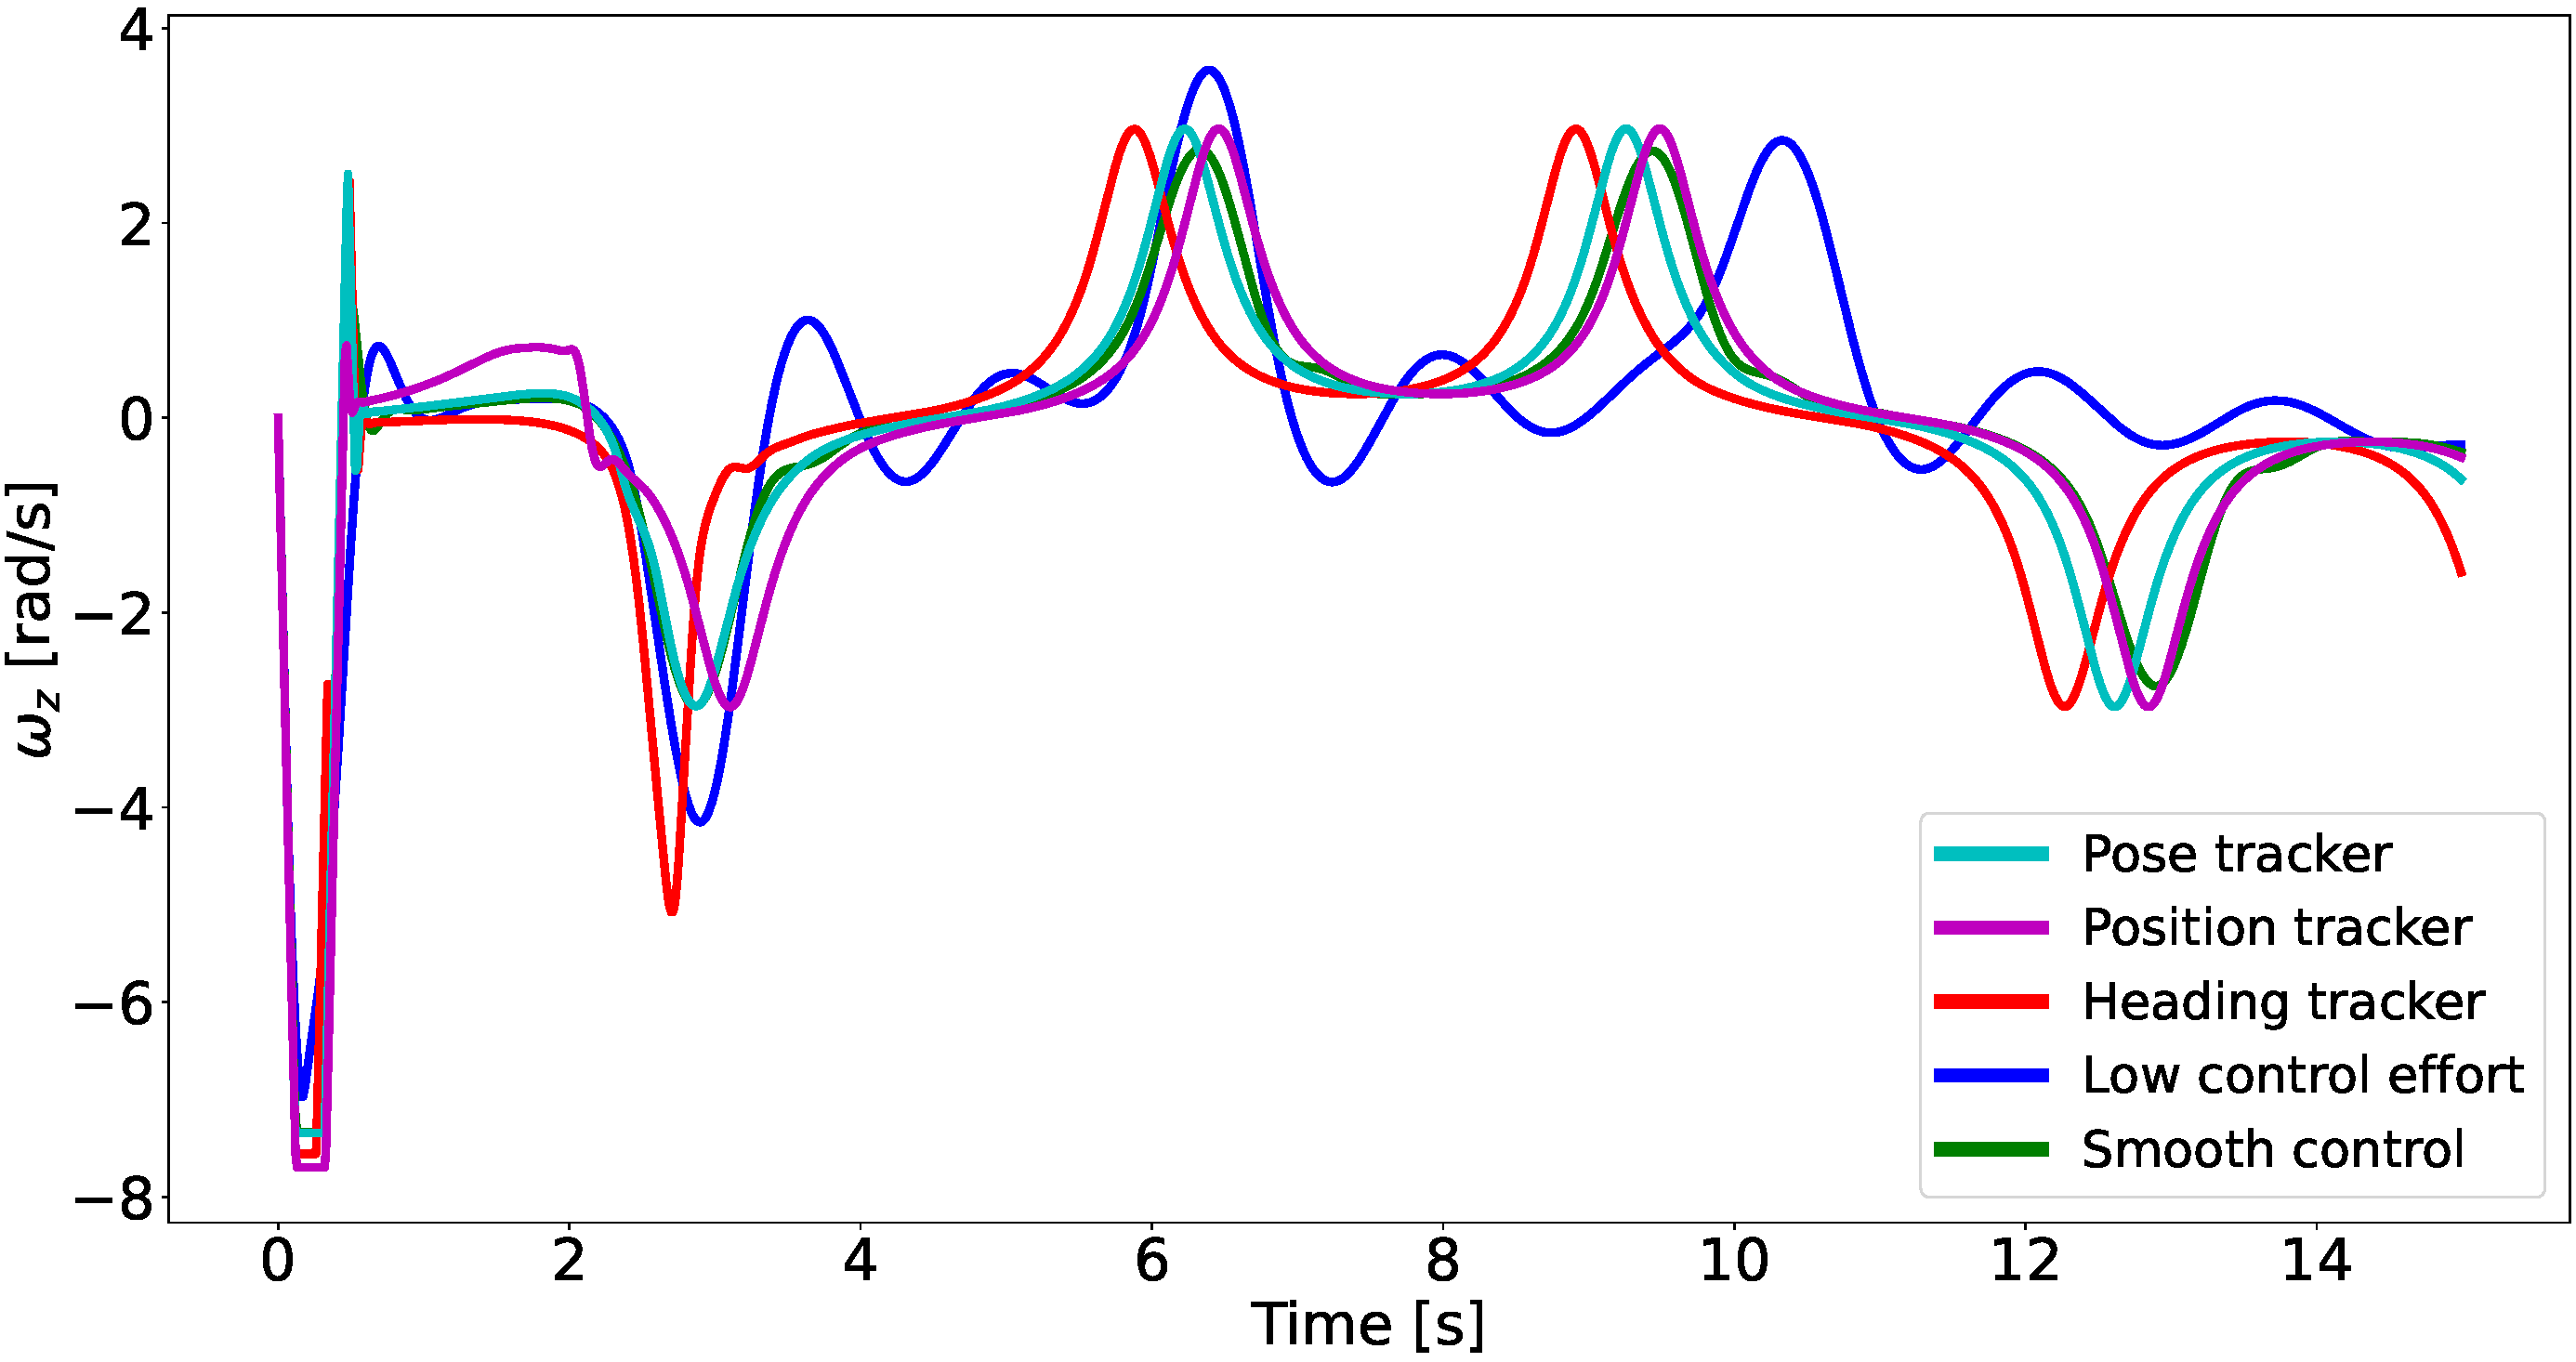
\includegraphics[width=0.48\textwidth]{Figures/One stage OCP/Solver specs comparison/Weights/Virtual speed controlled inside OCP/Planar_onestage_ocp_control_vspeed_comp_wz_weights.pdf}
        \label{subfig:PathTrackCompWeightsVarInsideVspeed_tr}
	}
	\hspace{-1.0em}
    \subfigure[Controlled virtual speed outside \acrshort{ocp}]{
        \centering
        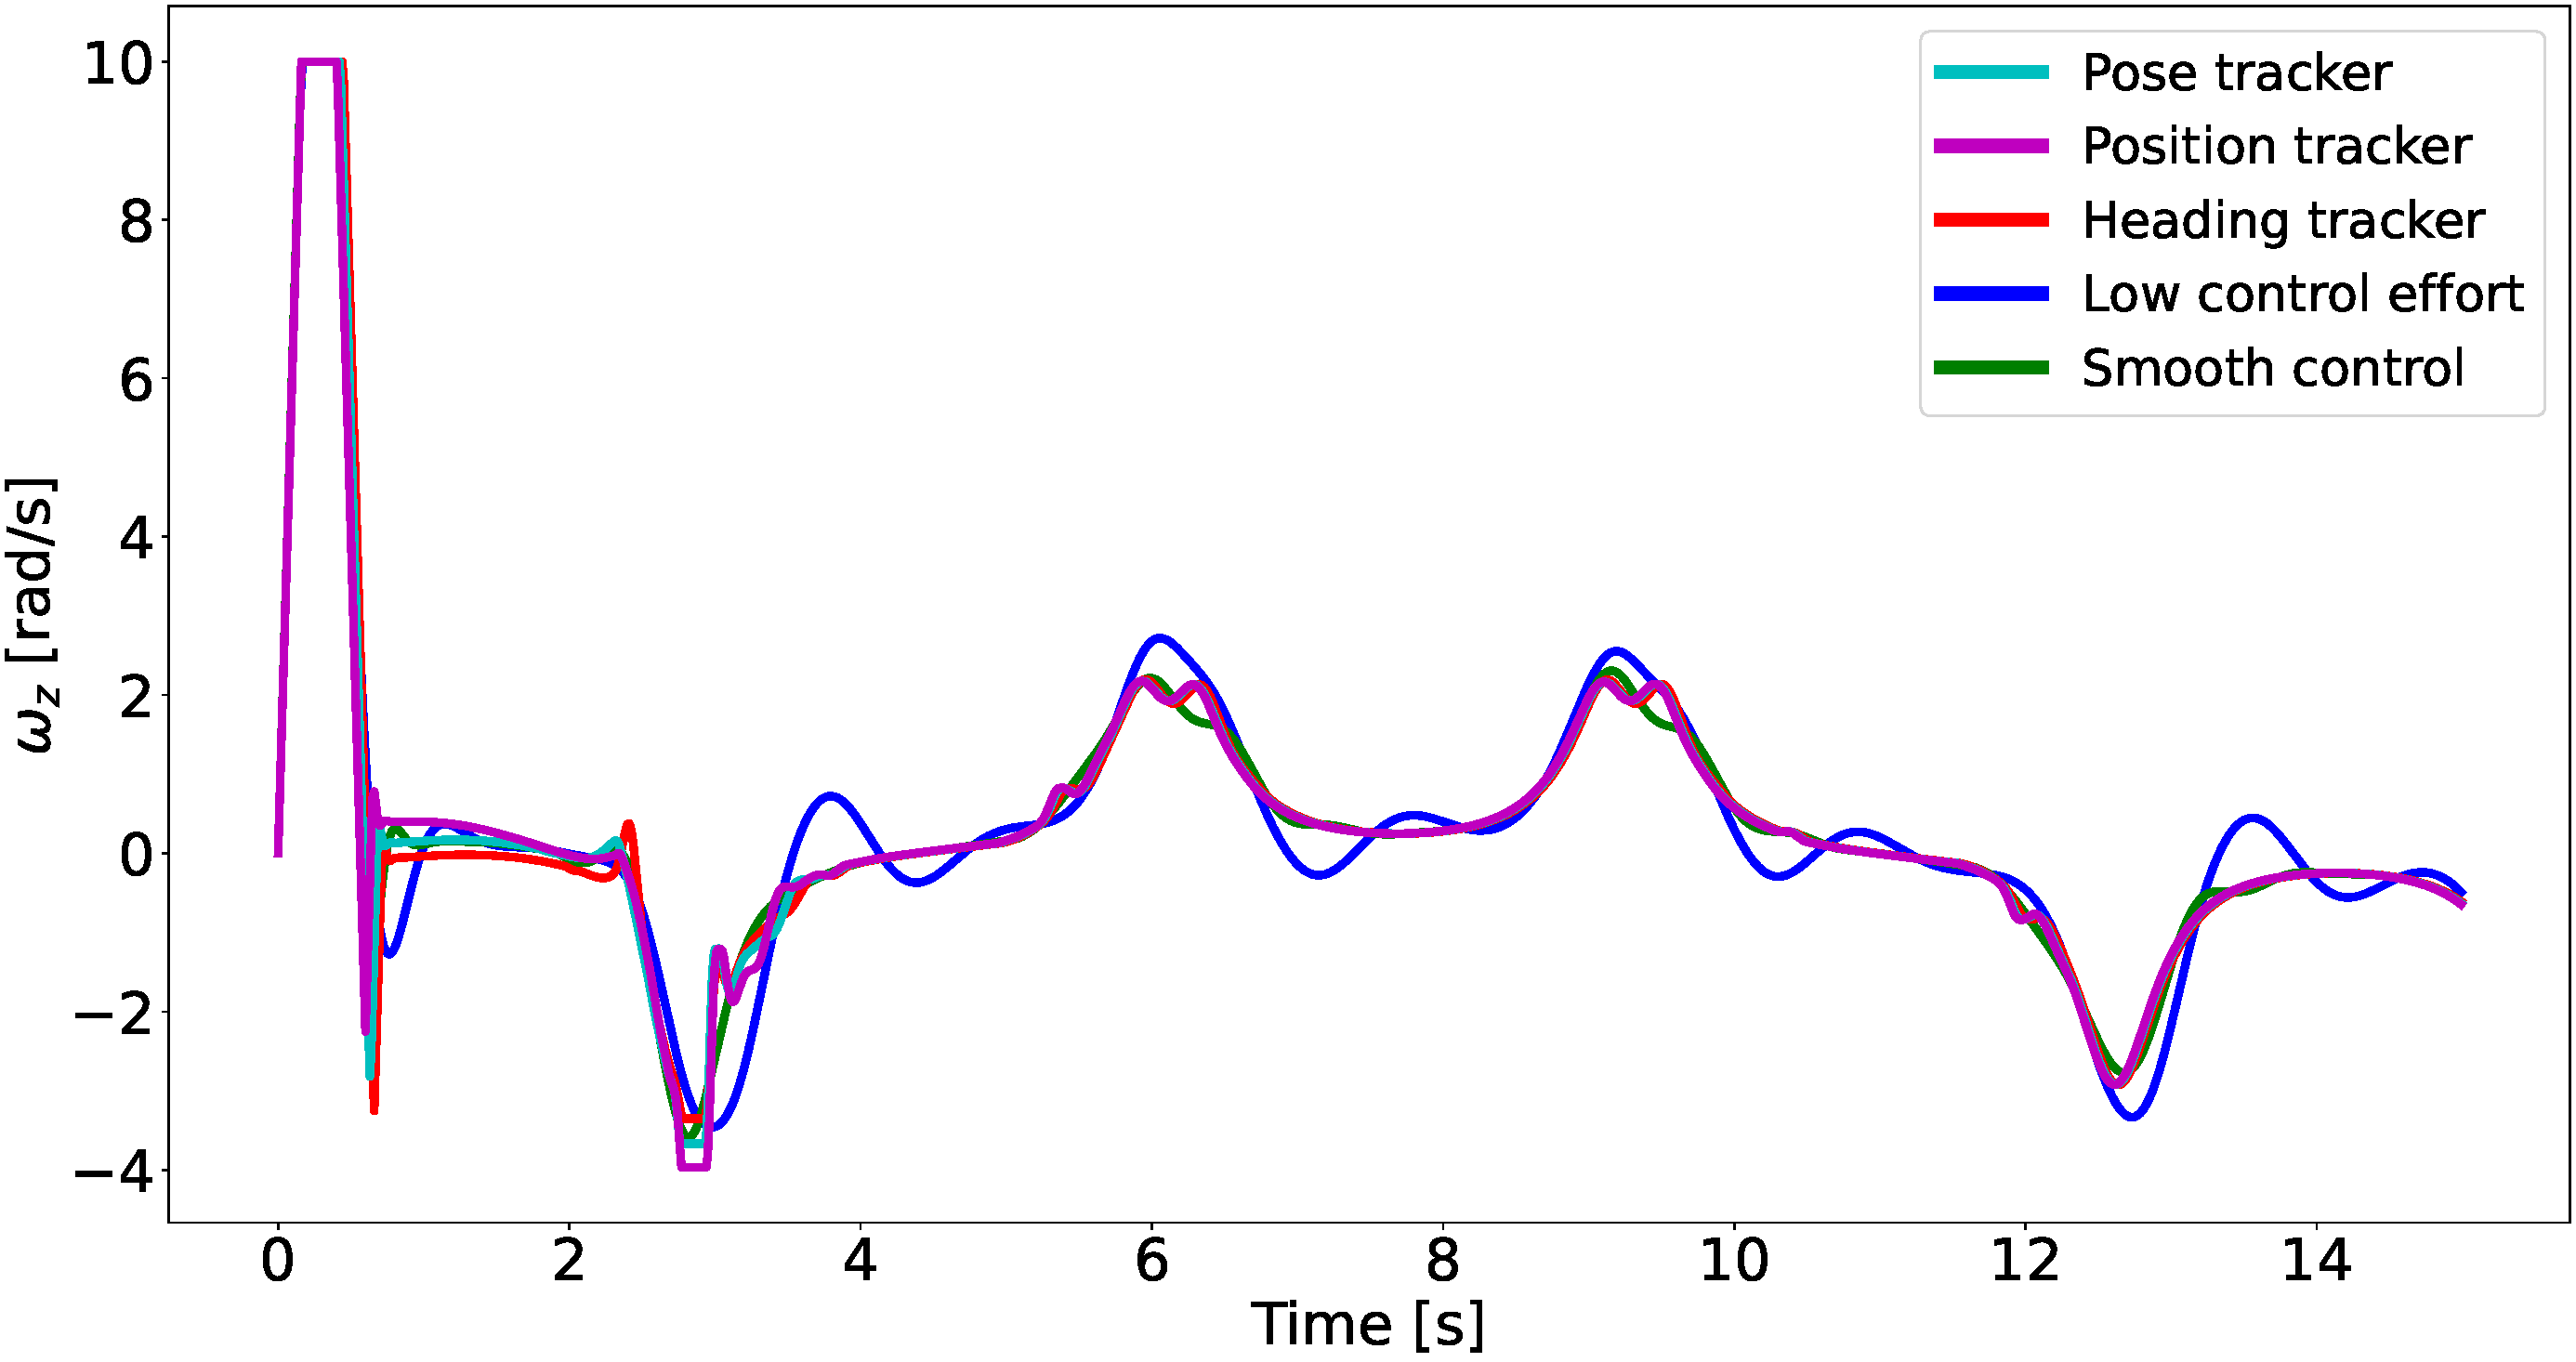
\includegraphics[width=0.48\textwidth]{Figures/One stage OCP/Solver specs comparison/Weights/Virtual speed controlled outside OCP/Planar_onestage_ocp_control_outside_vspeed_comp_wz_weights.pdf}
        \label{subfig:PathTrackCompWeightsVarOutsideVspeed_tr}
	}
	\caption{$\omega_z$ curve comparison among controllers.}
	\label{fig:PathTrackCompWeightsVar_wz}
\end{figure}

\begin{figure}[!htb]
	\centering
	\subfigure[Controlled virtual speed inside \acrshort{ocp}]{
        \centering
        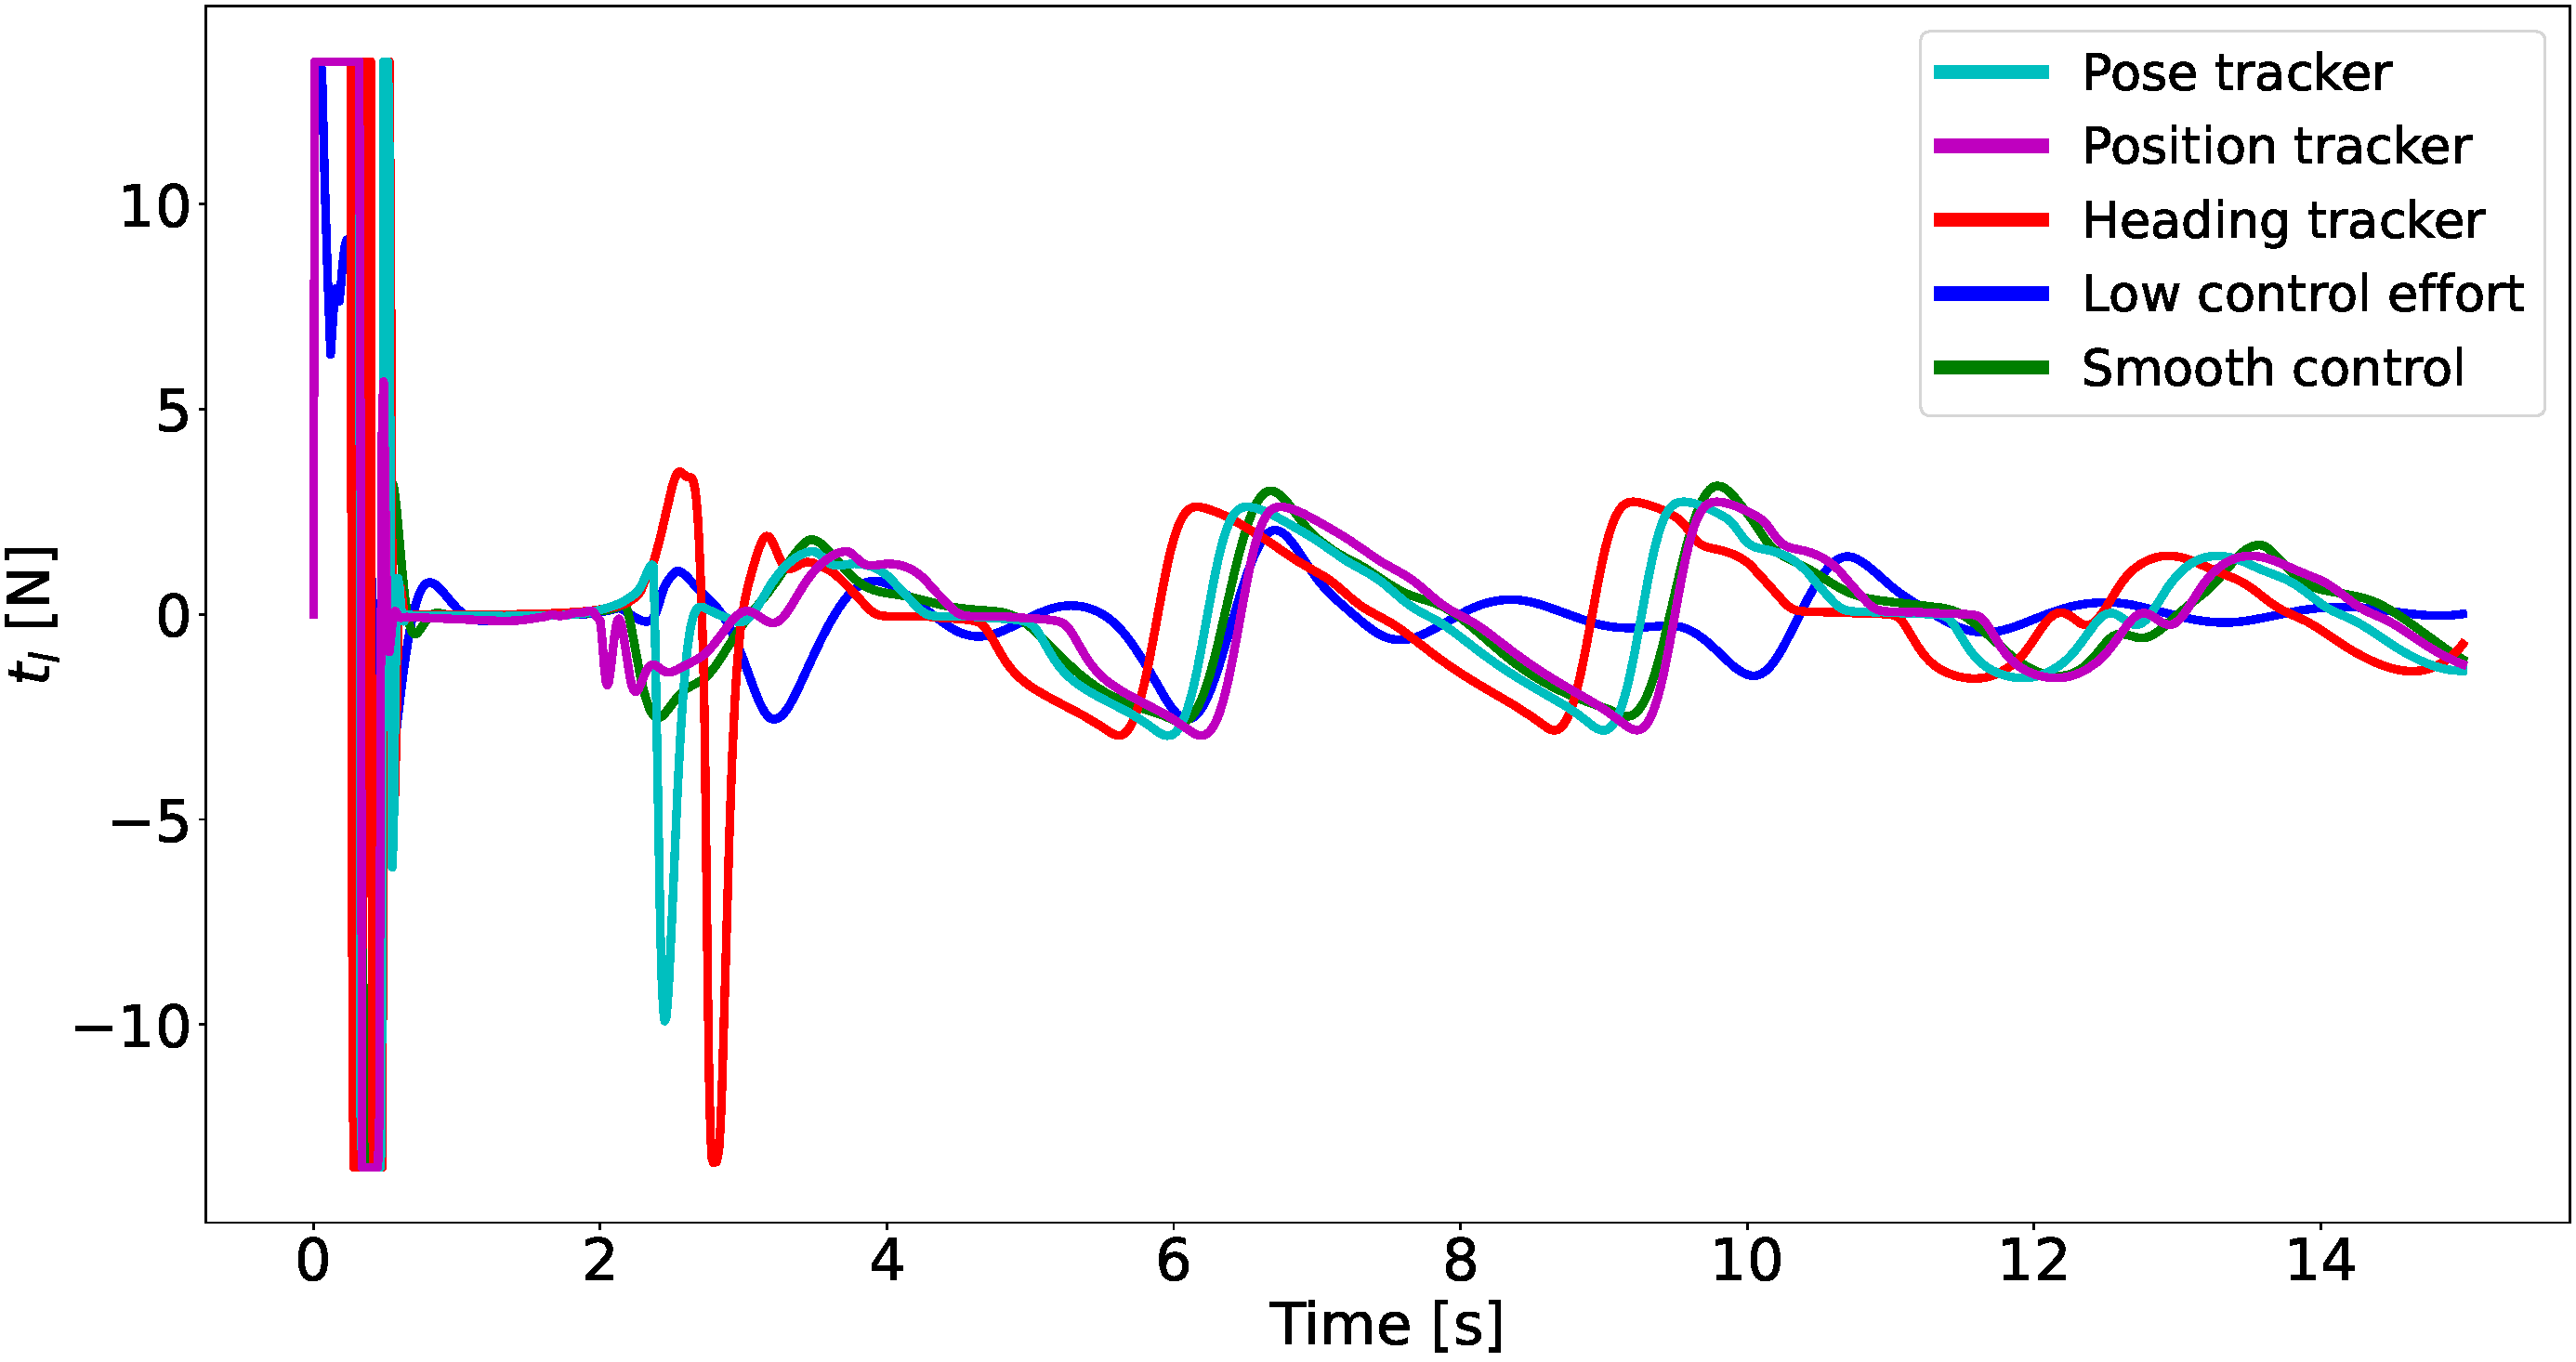
\includegraphics[width=0.48\textwidth]{Figures/One stage OCP/Solver specs comparison/Weights/Virtual speed controlled inside OCP/Planar_onestage_ocp_control_vspeed_comp_tl_weights.pdf}
        \label{subfig:PathTrackCompWeightsVarInsideVspeed_tl}
	}
	\hspace{-1.0em}
    \subfigure[Controlled virtual speed outside \acrshort{ocp}]{
        \centering
        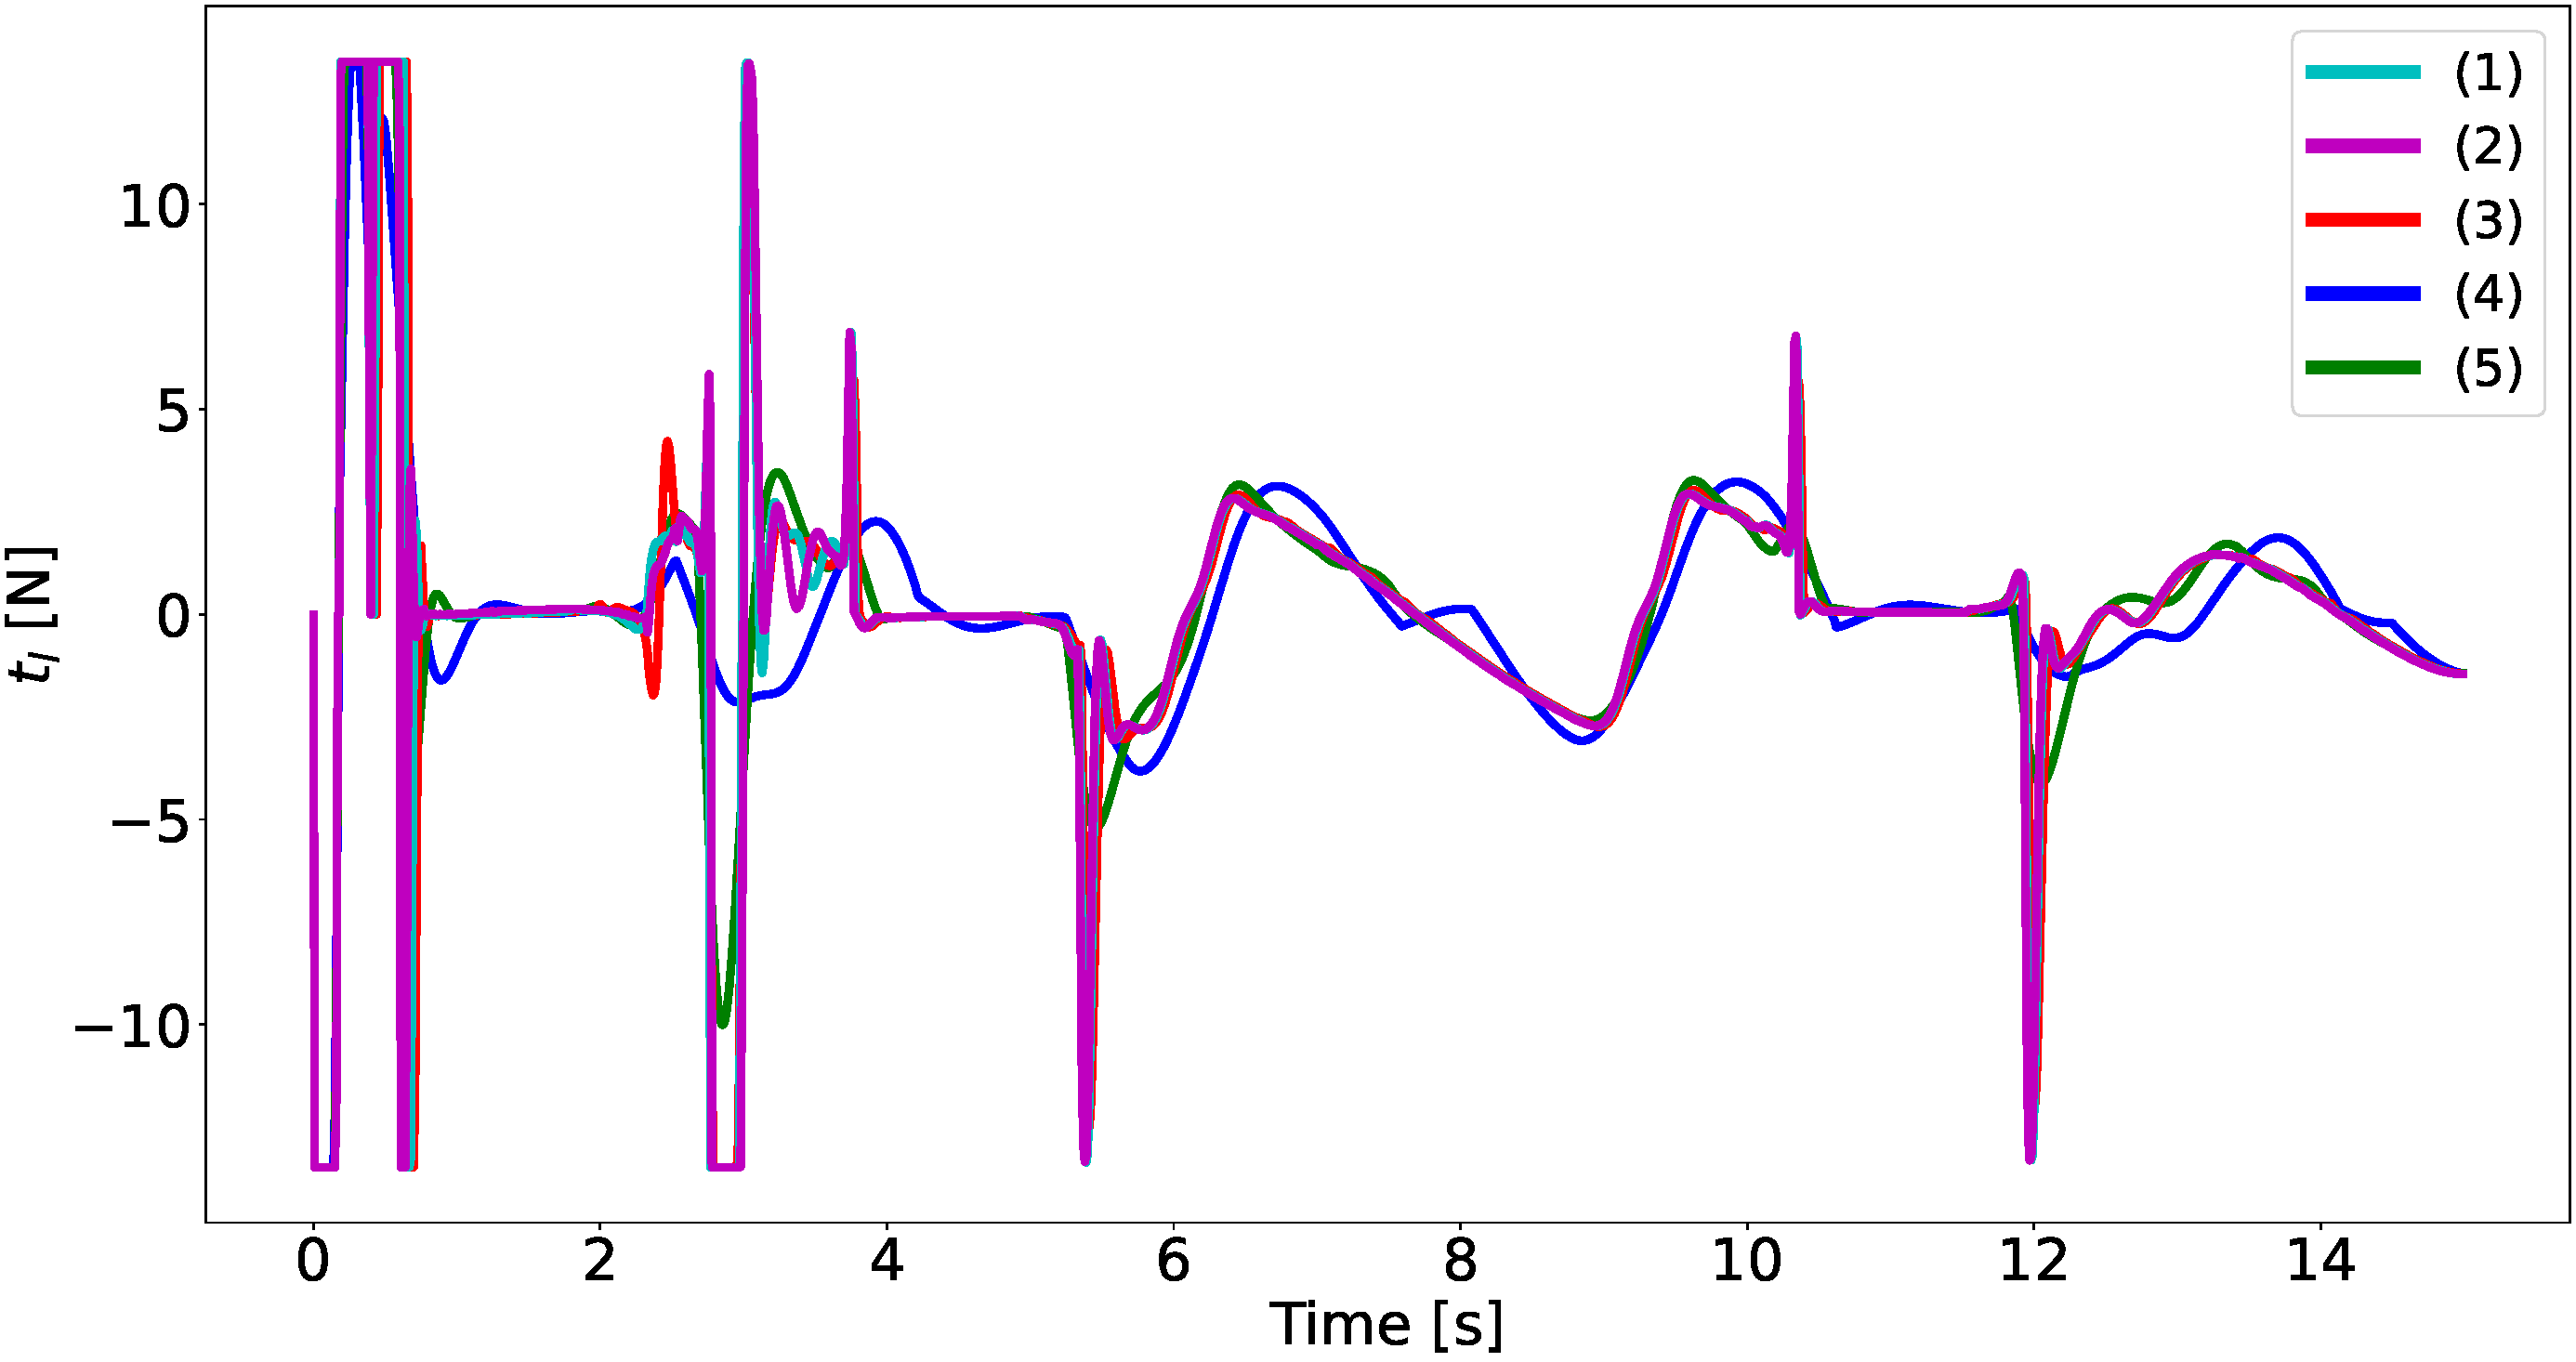
\includegraphics[width=0.48\textwidth]{Figures/One stage OCP/Solver specs comparison/Weights/Virtual speed controlled outside OCP/Planar_onestage_ocp_control_outside_vspeed_comp_tl_weights.pdf}
        \label{subfig:PathTrackCompWeightsVarOutsideVspeed_tl}
	}
	\caption{$\Traction_l$ curve comparison among controllers.}
	\label{fig:PathTrackCompWeightsVar_tl}
\end{figure}

\begin{figure}[!htb]
	\centering
	\subfigure[Controlled virtual speed inside \acrshort{ocp}]{
        \centering
        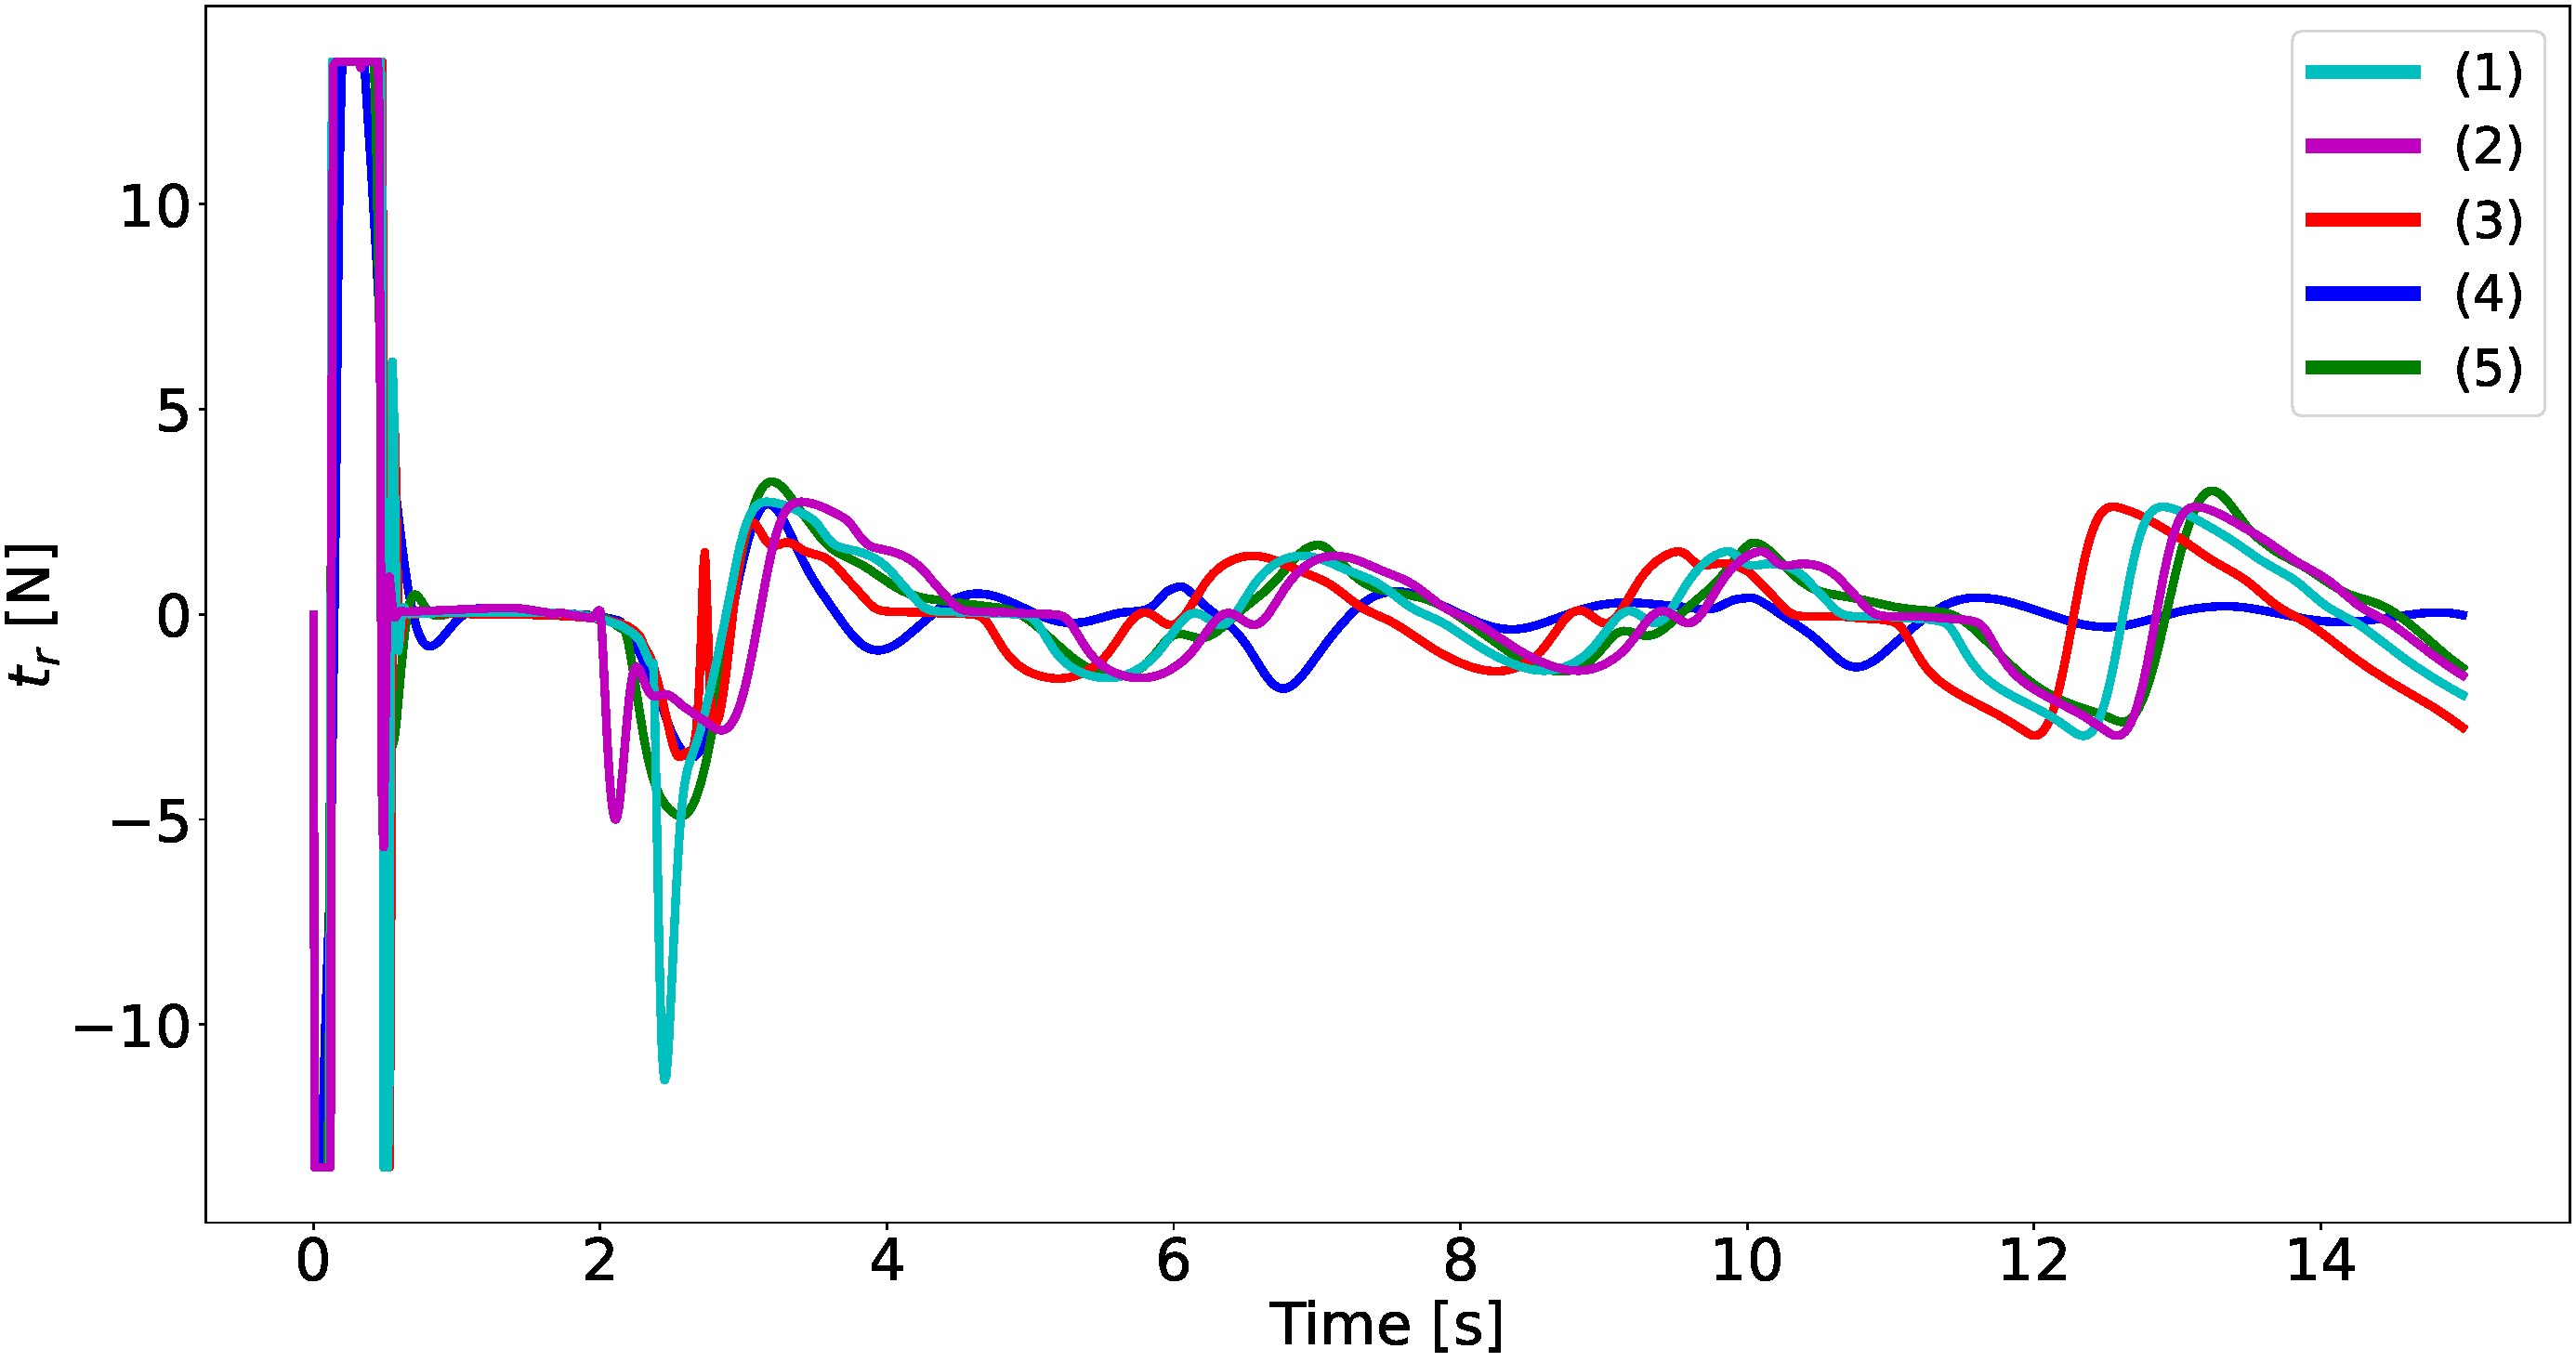
\includegraphics[width=0.48\textwidth]{Figures/One stage OCP/Solver specs comparison/Weights/Virtual speed controlled inside OCP/Planar_onestage_ocp_control_vspeed_comp_tr_weights.pdf}
        \label{subfig:PathTrackCompWeightsVarInsideVspeed_tr}
	}
	\hspace{-1.0em}
    \subfigure[Controlled virtual speed outside \acrshort{ocp}]{
        \centering
        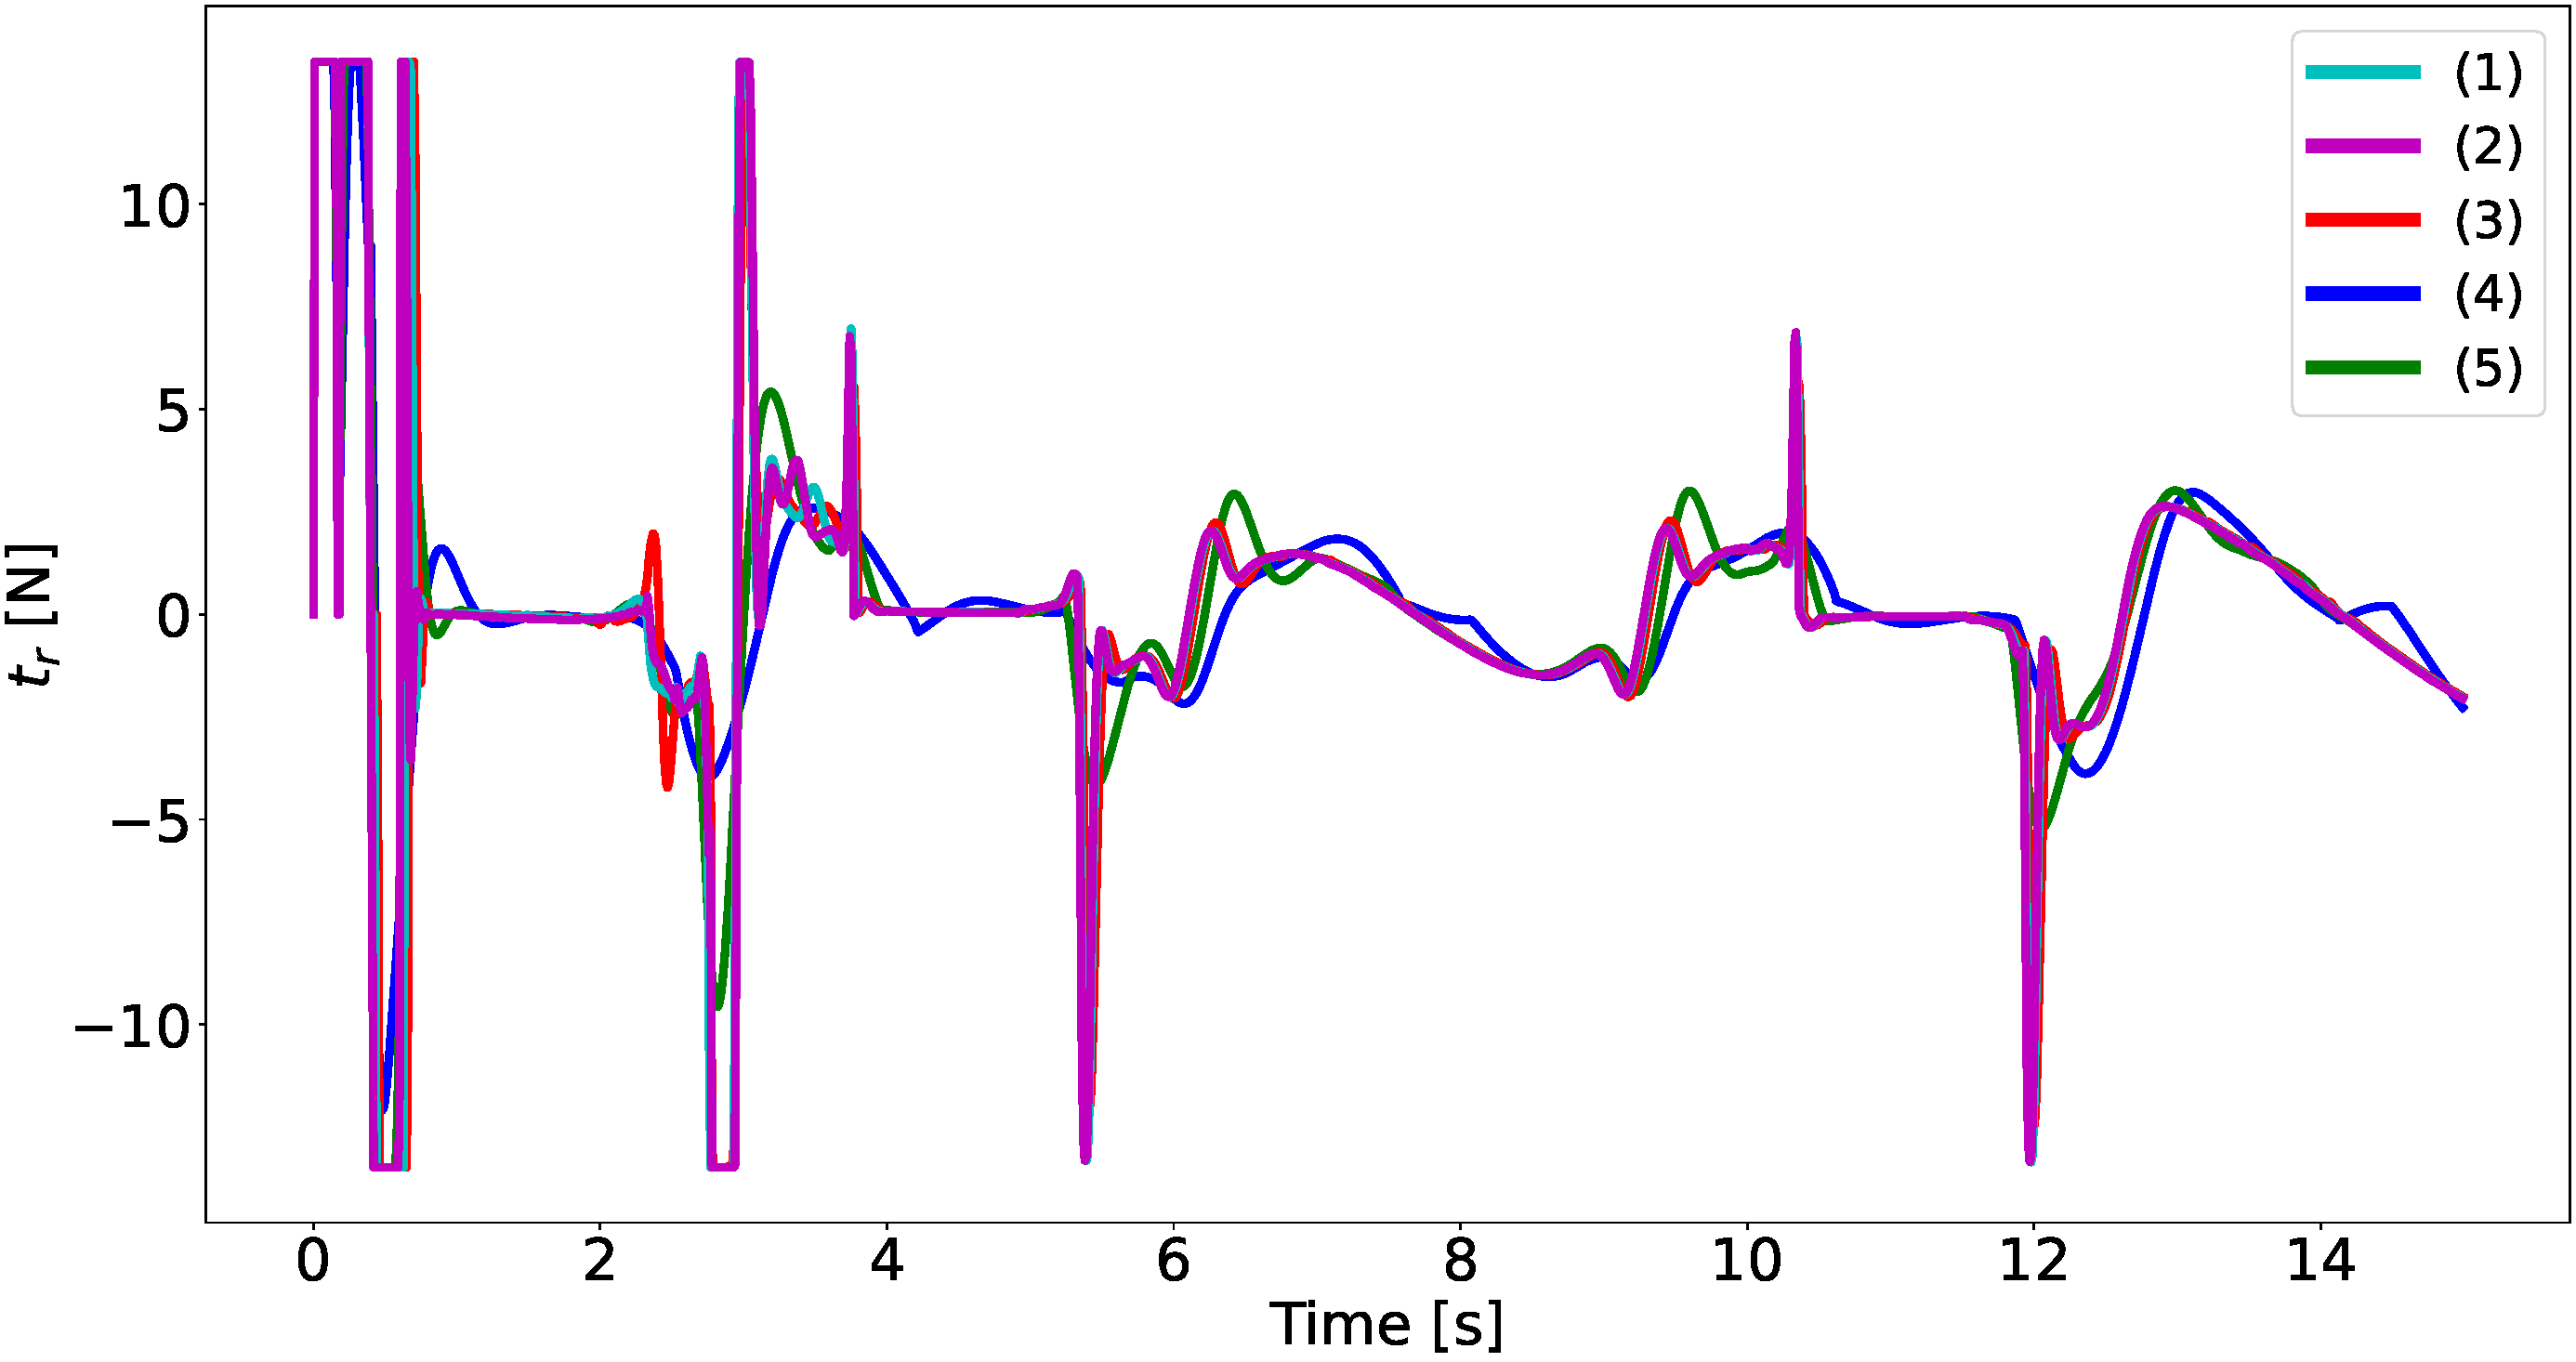
\includegraphics[width=0.48\textwidth]{Figures/One stage OCP/Solver specs comparison/Weights/Virtual speed controlled outside OCP/Planar_onestage_ocp_control_outside_vspeed_comp_tr_weights.pdf}
        \label{subfig:PathTrackCompWeightsVarOutsideVspeed_tr}
	}
	\caption{$\Traction_r$ curve comparison among controllers .}
	\label{fig:PathTrackCompWeightsVar_tr}
\end{figure}

\subsection{Real-time one-stage \acrshort{ocp} on rough, uneven terrain}
\label{subsection:realtimeonestageocpRoughUnevenTerrain}

\subsubsection*{Reference tour}

The results of the reference tour are presented below. Solver $(3)$ is applied and has proven to be computionally feasible and to deliver low cost feedbacks. The reference heading is followed and slippage only arises at the highest inclinations. The traction rates only reach unusual values where there is a need to correct for a $\pi\,[rad]$ deviation of the mobile robot in the beginning. After this initial correction, the solver completely focuses on balancing the mobile robot and tracking the reference. Among $100000$ simulation iterations, the solver only fails on $0.014\,\%$ of the iterations and slippage only happens on $0.026\,\%$ of the iterations. $4$ timeouts were recorded. 

Along the reference tour, the recorded loop time and optimal cost are $7.4 \pm 2.0\,[ms]$ and $0.26 \pm 5.26$, respectively. The first number is the average and the second is the standard deviation.

\begin{figure}[!htb]
  \begin{subfigmatrix}{4}
    \subfigure[Loop time along reference.]{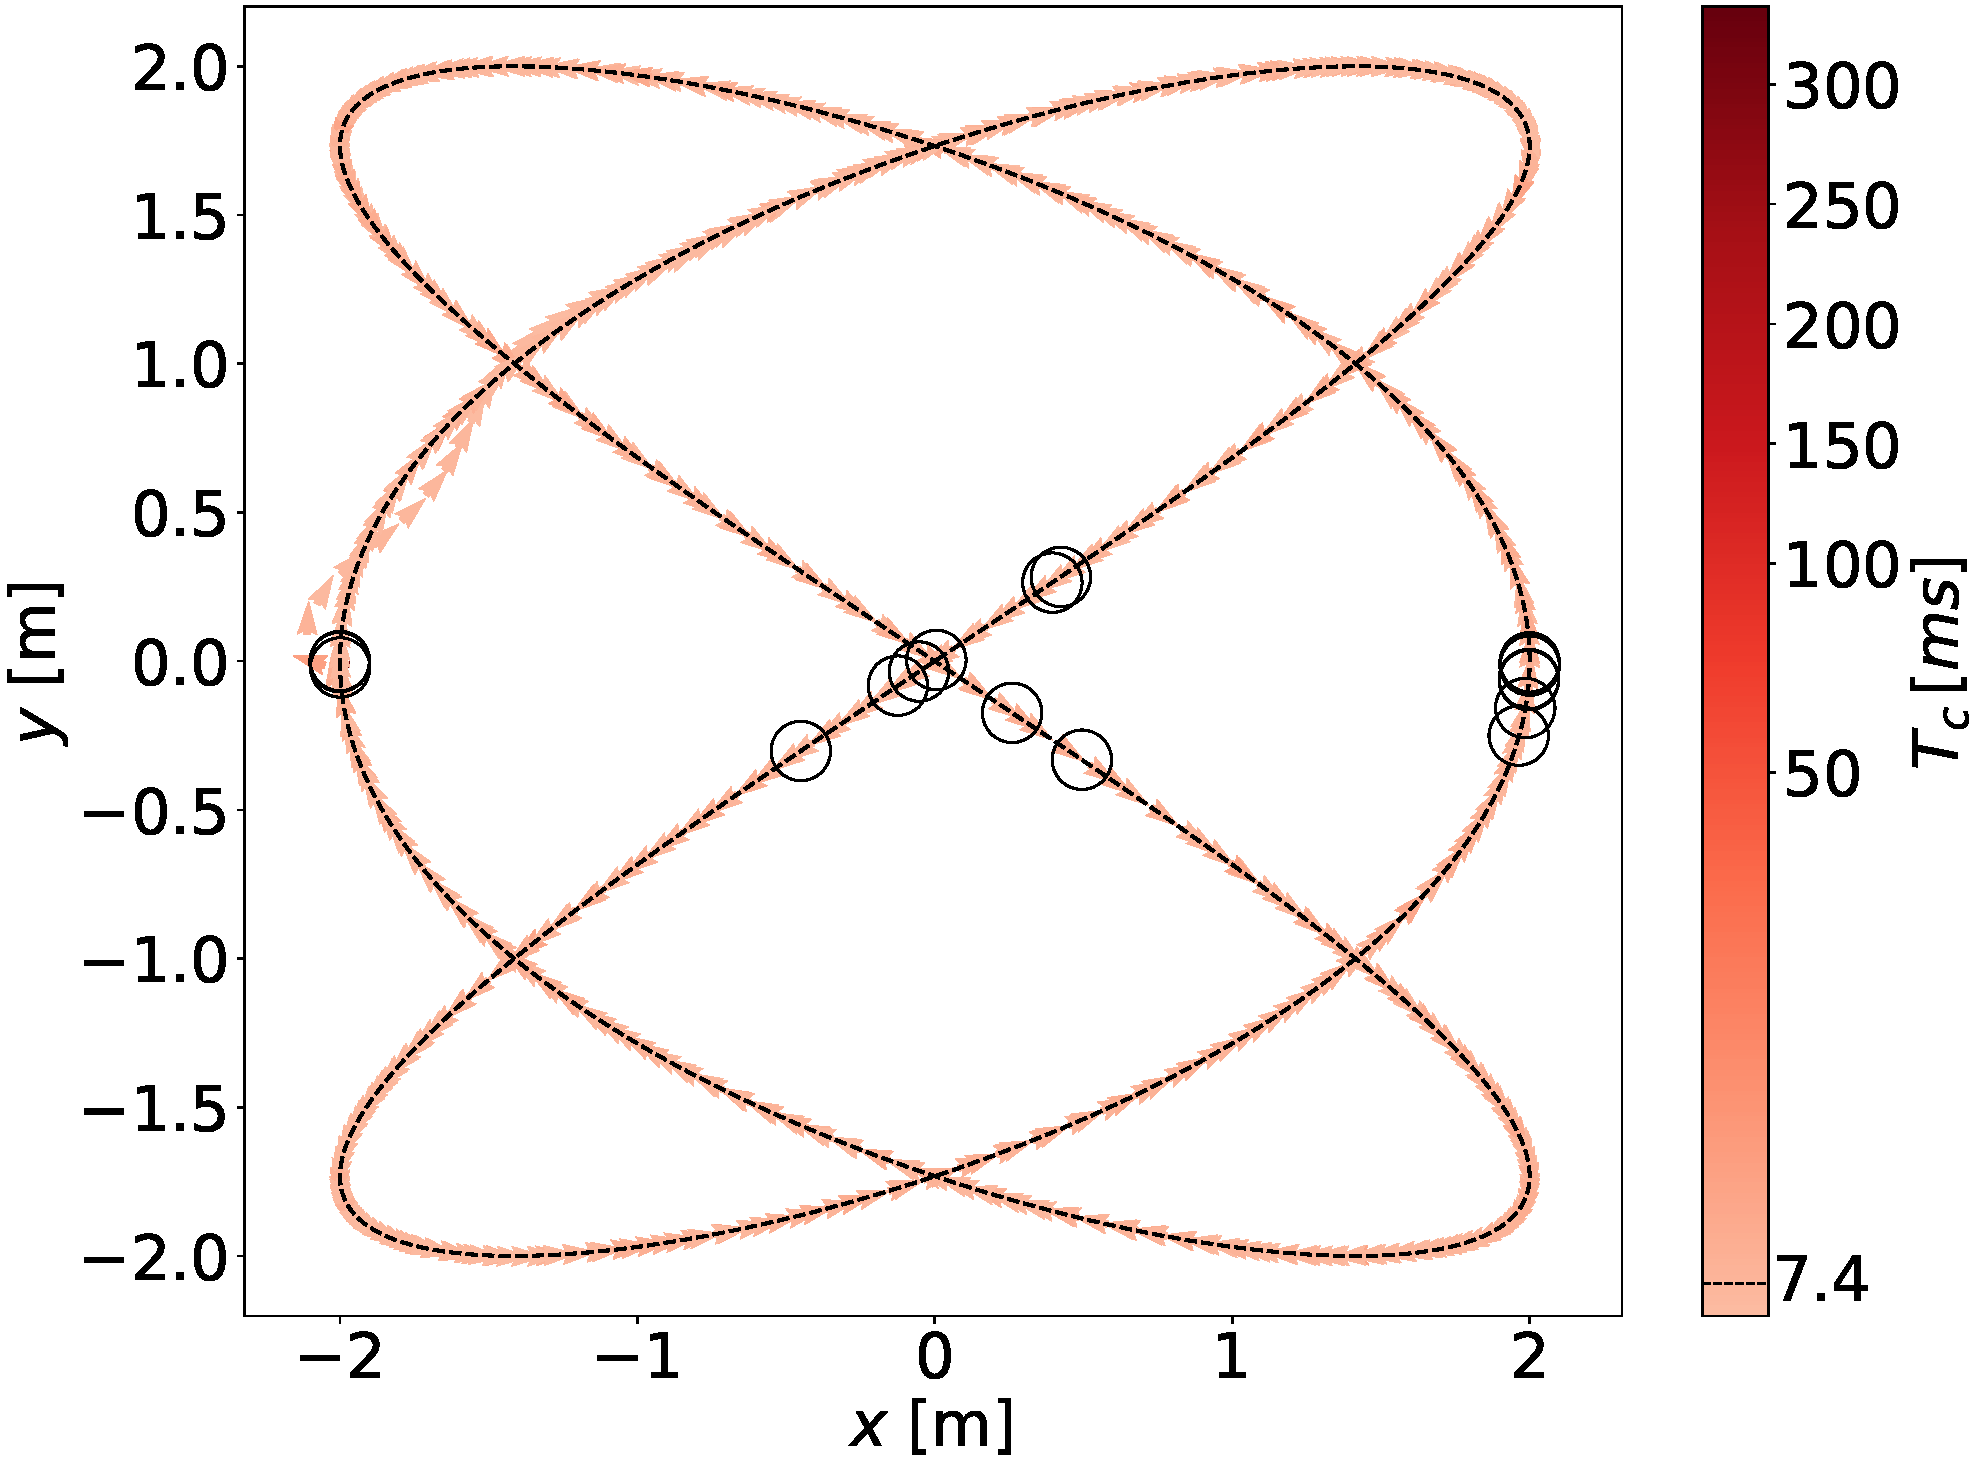
\includegraphics[width=0.49\linewidth]{Figures/Real time one stage OCP on rough terrain/Rough and uneven terrain map/reference_tour_opt_time.pdf}}
    \subfigure[Optimal cost along reference.]{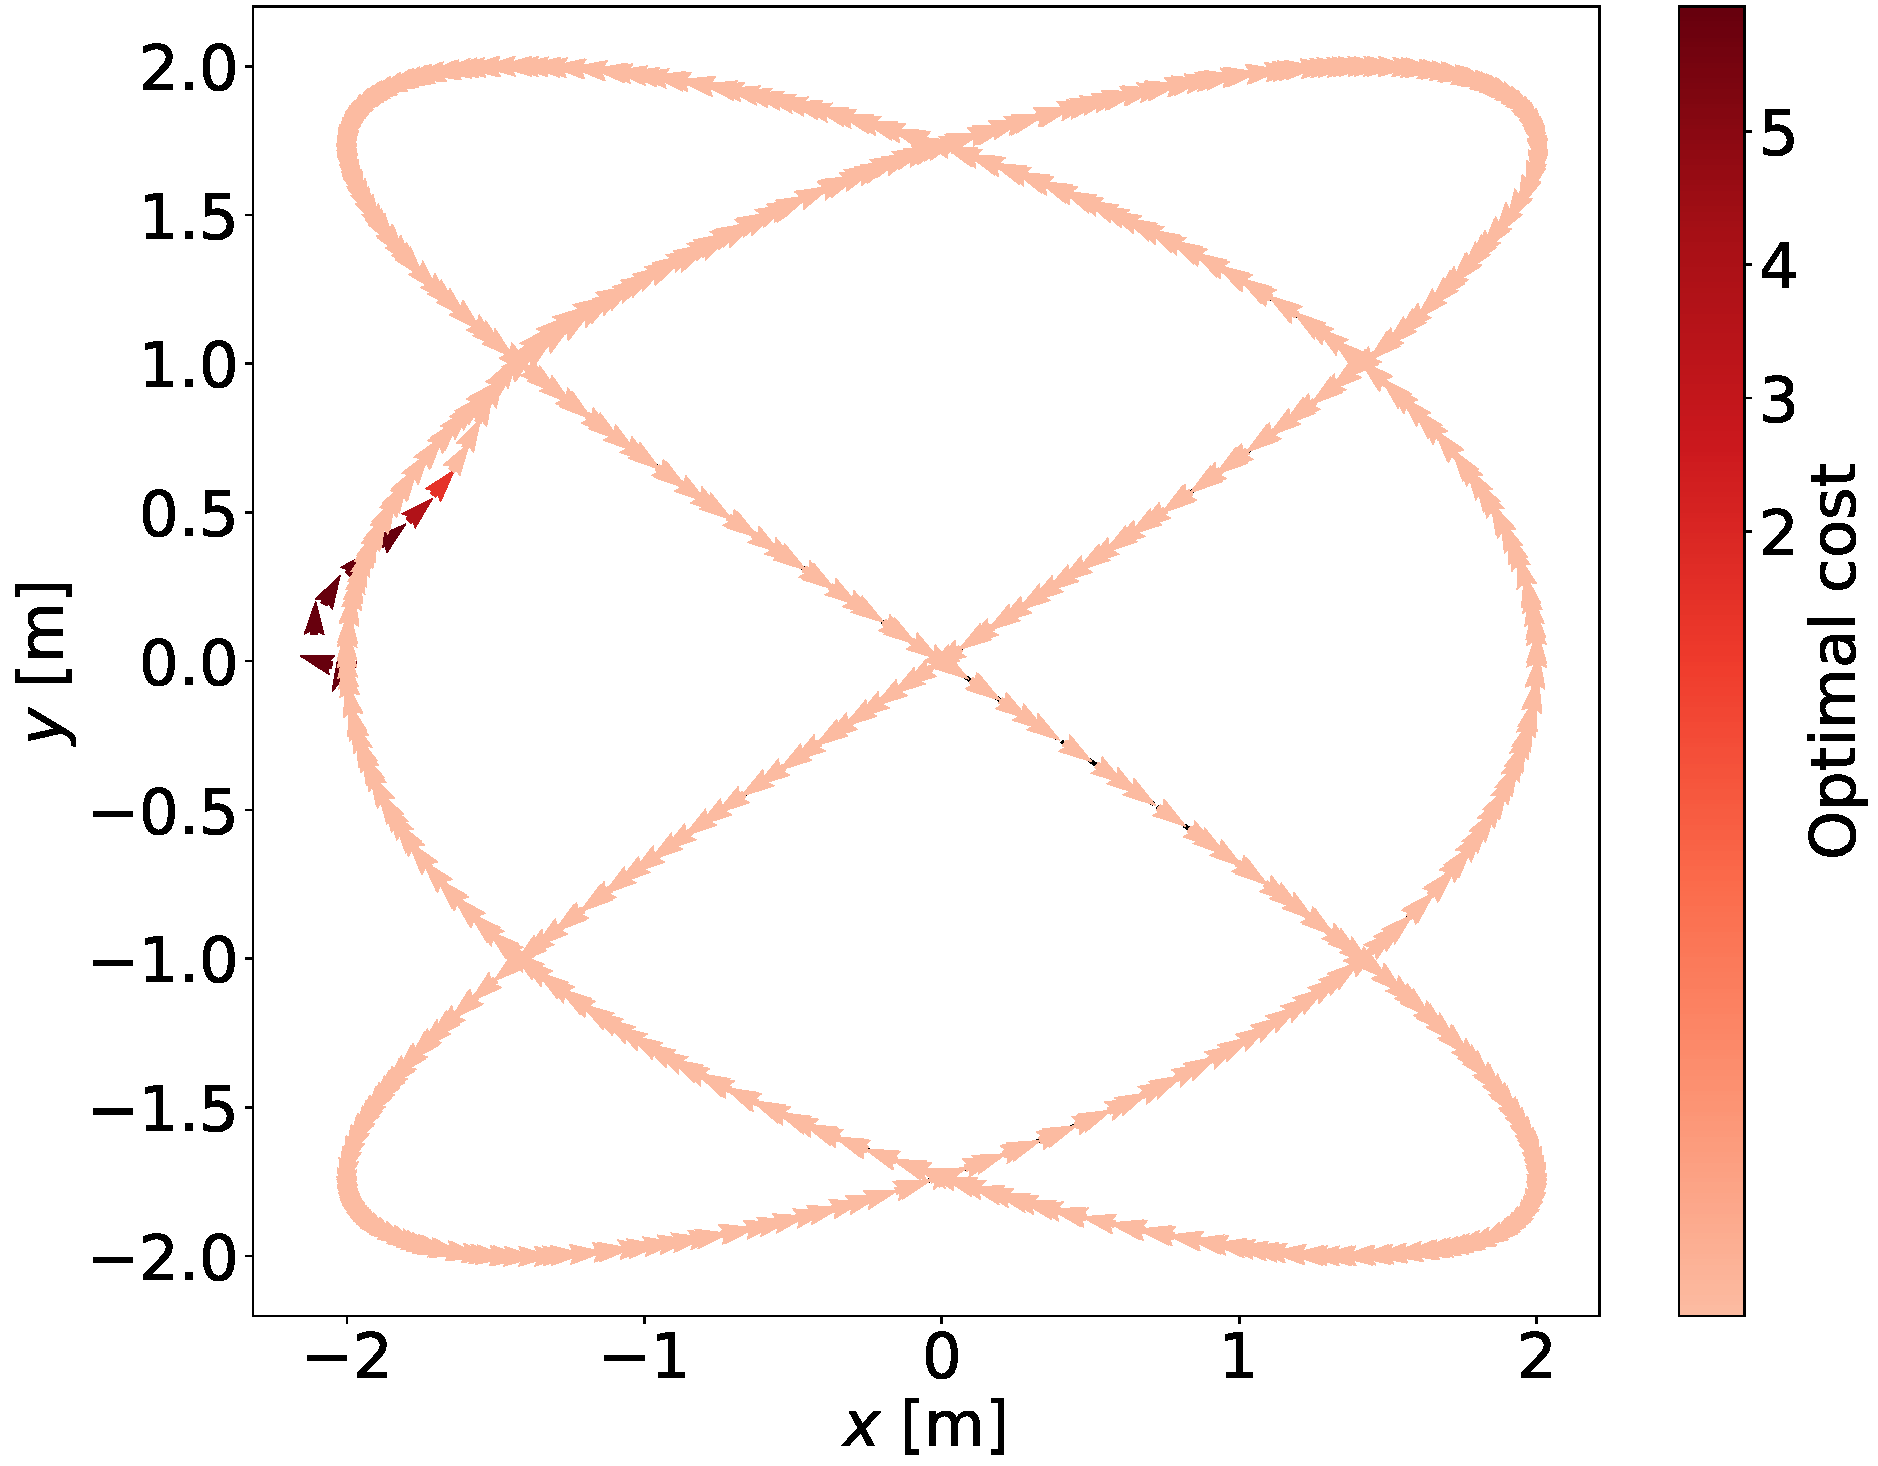
\includegraphics[width=0.49\linewidth]{Figures/Real time one stage OCP on rough terrain/Rough and uneven terrain map/reference_tour_opt_cost.pdf}}
    \subfigure[Traction forces on friction cone.]{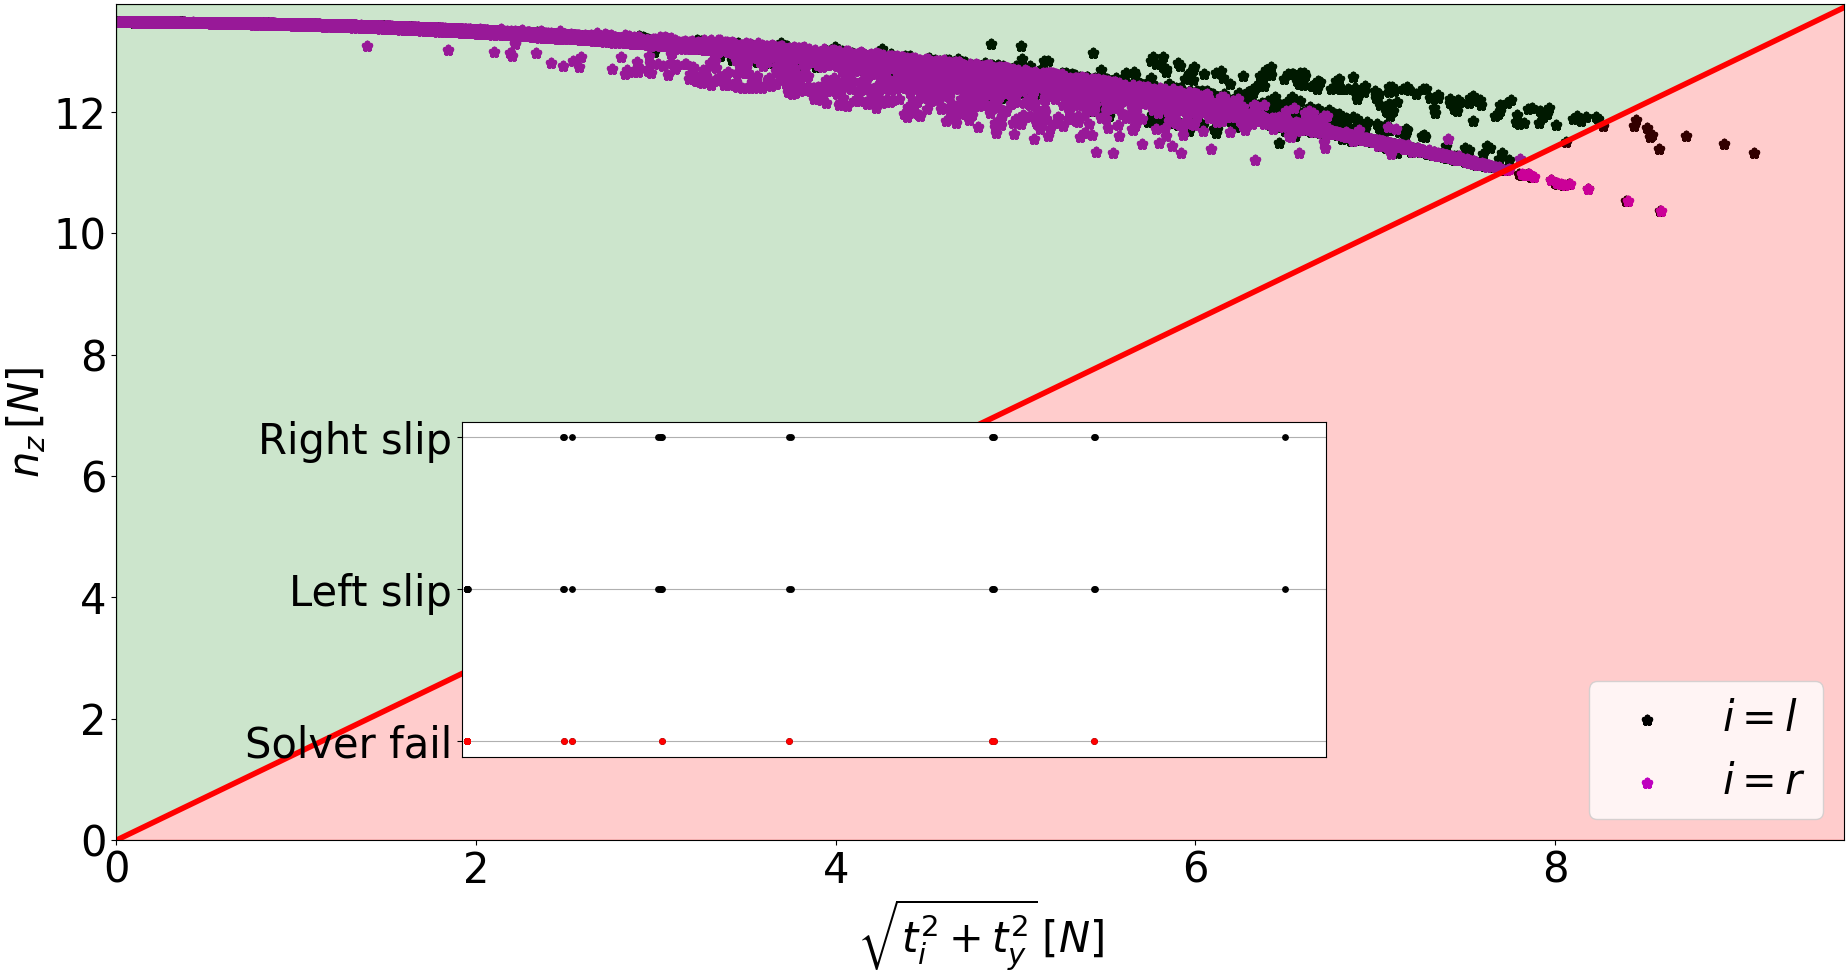
\includegraphics[width=0.49\linewidth]{Figures/Real time one stage OCP on rough terrain/Rough and uneven terrain map/reference_tour_forces_cone.png}}
    \subfigure[Traction rates along simulation.]{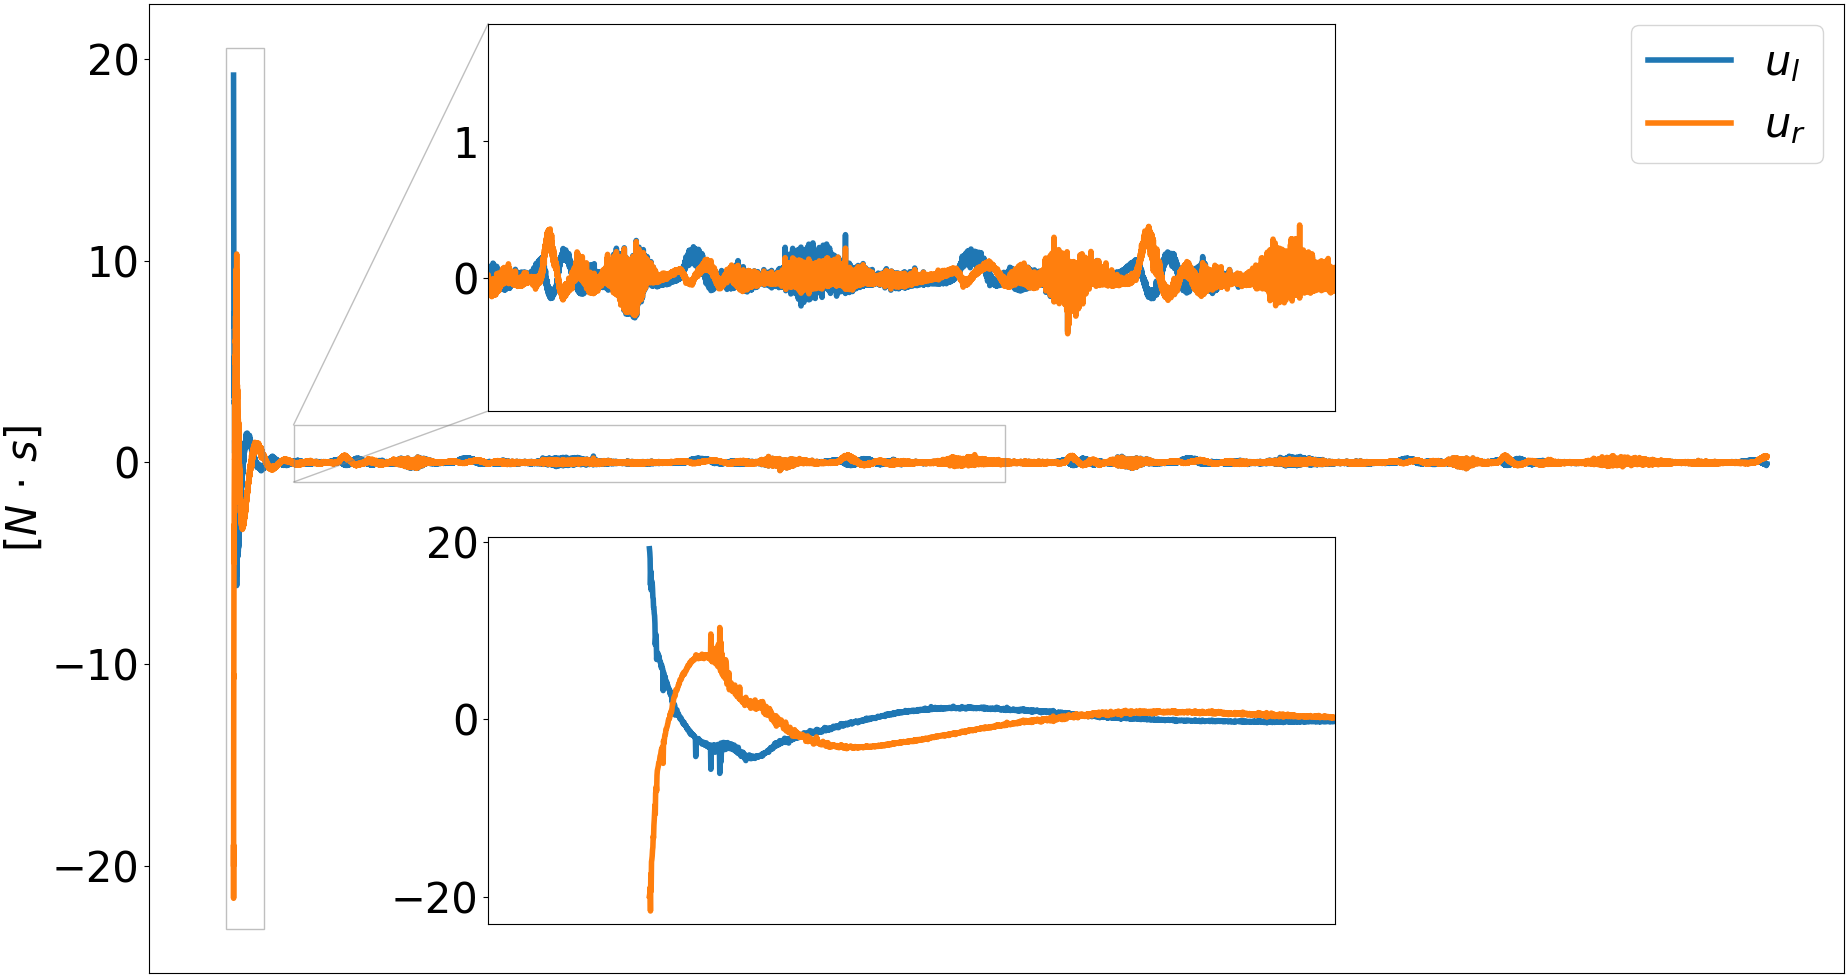
\includegraphics[width=0.49\linewidth]{Figures/Real time one stage OCP on rough terrain/Rough and uneven terrain map/reference_tour_forces_rate_curve.png}}
  \end{subfigmatrix}
  \caption{Reference tour.}
  \label{fig:referenceTourStats}
\end{figure}

In figure \ref{fig:referenceTourStats}, the black circles on the top left picture denote the places where slippage takes place. On the bottom left picture, the white window denotes the iterations where slippage or solver fail was recorded.